\documentclass[12pt]{article}
\usepackage{listings}
\usepackage{color} %red, green, blue, yellow, cyan, magenta, black, white
\definecolor{mygreen}{RGB}{28,172,0} % color values Red, Green, Blue
\definecolor{mylilas}{RGB}{170,55,241}
\usepackage{listings}
\usepackage{qtree}
\usepackage[T1]{fontenc}
\usepackage{indentfirst}
\usepackage{booktabs,amsmath}
\usepackage{amsfonts}
\usepackage[utf8]{inputenc}
\usepackage{amssymb}
\usepackage{graphicx}
\usepackage{xcolor}
\usepackage{float}
\usepackage[bottom]{footmisc}
\usepackage[hidelinks,bookmarks=false]{hyperref}
\usepackage{epstopdf}
\usepackage{footnotebackref}
\usepackage{enumitem}
\usepackage{xcolor}
\usepackage{multirow}
\usepackage{tabularx}
\usepackage{bbm}
\usepackage{mathtools}
\usepackage{bm}
\usepackage{esvect}
\newcommand\myworries[1]{\textcolor{red}{#1}}
\newcommand\mythoughts[1]{\textcolor{blue}{#1}}
\newcommand\independent{\protect\mathpalette{\protect\independenT}{\perp}}
\def\independenT#1#2{\mathrel{\rlap{$#1#2$}\mkern2mu{#1#2}}}
\usepackage{hyperref}
\usepackage{scalerel,stackengine}
\stackMath
\newcommand\reallywidehat[1]{%
\savestack{\tmpbox}{\stretchto{%
  \scaleto{%
    \scalerel*[\widthof{\ensuremath{#1}}]{\kern-.6pt\bigwedge\kern-.6pt}%
    {\rule[-\textheight/2]{1ex}{\textheight}}%WIDTH-LIMITED BIG WEDGE
  }{\textheight}% 
}{0.5ex}}%
\stackon[1pt]{#1}{\tmpbox}%
}
\parskip 1ex
\hypersetup{
	colorlinks,
	linkcolor={red!50!black},
	citecolor={red!80!black},
	urlcolor={blue!80!black},
	pdfstartview={}
}
\usepackage{dirtytalk}
\newcommand\norm[1]{\left\lVert#1\right\rVert}
\usepackage{lmodern}
\usepackage{booktabs, caption, makecell}
\usepackage{threeparttable}
\usepackage[round, authoryear]{natbib}
\bibliographystyle{rusnat}
\usepackage[left=2.5cm,right=2.5cm,top=2.5cm,bottom=2.5cm]{geometry}
\newtheorem{theorem}{Theorem}
\newtheorem{acknowledgement}{Acknowledgement}
\newtheorem{algorithm}{Algorithm}
\newtheorem{assumption}{Assumption}
\newtheorem{axiom}{Axiom}
\newtheorem{case}{Case}
\newtheorem{claim}{Claim}
\newtheorem{conclusion}{Conclusion}
\newtheorem{condition}{Condition}
\newtheorem{conjecture}{Conjecture}
\newtheorem{corollary}{Corollary}
\newtheorem{criterion}{Criterion}
\newtheorem{definition}{Definition}
\newtheorem{example}{Example}
\newtheorem{exercise}{Exercise}
\newtheorem{lemma}{Lemma}
\newtheorem{notation}{Notation}
\newtheorem{problem}{Problem}
\newtheorem{Proof of Lemma}{Proof of Lemma}
\newtheorem{proposition}{Proposition}
\newtheorem{remark}{Remark}
\newtheorem{solution}{Solution}
\newtheorem{summary}{Summary}
\newenvironment{proof}[1][Proof]{\noindent\textbf{#1.} }{\ \rule{0.5em}{0.5em}}
\usepackage{setspace}
\onehalfspacing
\lstset{basicstyle=\footnotesize\ttfamily,breaklines=true}
\lstset{framextopmargin=50pt,frame=bottomline}

\DeclareMathOperator*{\argmax}{arg\,max}
\DeclareMathOperator*{\argmin}{arg\,min}

\title{CompSci671 Final Project: Trading at the Close \\}
\author{Qijun Yang}
\date{ Dec 5th 2023\\}

\usepackage{hyperref}
\usepackage{graphicx}

\begin{document}

\maketitle


\section{Background}
\subsection{Introduction}

The stock market is a dynamic and high-pressure environment, where every second can be pivotal. This is especially true in the final moments of a trading session. The last ten minutes often witness heightened market volatility and rapid fluctuations in stock prices, playing a critical role in shaping the day's economic narrative globally.

A key event in the Nasdaq Stock Exchange's trading day is the Nasdaq Closing Cross auction. This procedure determines the closing prices for stocks listed on the exchange, figures that are vital for investors, market analysts, and other stakeholders in evaluating the performance of individual stocks and the market at large.

Predicting closing price movements is a crucial task for market makers, as it enhances market efficiency and accessibility, especially during the trading day's intense final ten minutes.

Leveraging data from the order book and the closing auction of the stock provided by the \href{https://www.kaggle.com/competitions/optiver-trading-at-the-close/overview}{Optiver Kaggle competition}, along with the knowledge acquired in this course, I aim to develop models that not only predict closing price movements of Nasdaq-listed stocks with high accuracy but also offer clear \textbf{interpretability}. This approach aligns with the need for transparent and explainable AI in financial markets.



\subsection{Data Description \& Exploratory Data Analysis}

\subsubsection*{Dataset Source} \href{https://www.kaggle.com/competitions/optiver-trading-at-the-close/data}{Optiver - Trading at the Close}

\subsubsection*{Key variables in Dataset}
The dataset consists of historical data from the daily ten-minute closing auction on the NASDAQ stock exchange.
\begin{itemize}
  \item \texttt{stock\_id}: A unique identifier for the stock.
  \item \texttt{date\_id}: A unique identifier for the date.
  \item \texttt{imbalance\_size}: The amount unmatched at the current reference price (in USD).
  \item \texttt{imbalance\_buy\_sell\_flag}: An indicator reflecting the direction of auction imbalance.
  \item \texttt{reference\_price}: The near price bounded between the best bid and ask price.
  \item \texttt{matched\_size}: The amount that can be matched at the current reference price (in USD).
  \item \texttt{far\_price}: The crossing price that will maximize the number of shares matched based on auction interest only.
  \item \texttt{near\_price}: The crossing price that will maximize the number of shares matched based auction and continuous market orders.
  \item \texttt{[bid/ask]\_price} - Price of the most competitive buy/sell level in the non-auction book.
  \item \texttt{[bid/ask]\_size} - The dollar notional amount on the most competitive buy/sell level in the non-auction book.
  \item \texttt{wap} - The weighted average price in the non-auction book.
  \item \texttt{seconds\_in\_bucket} - The number of seconds elapsed since the beginning of the day's closing auction, always starting from 0.
  \item \texttt{target}: The 60-second future move in the weighted average price of the stock, less the 60-second future move of the synthetic index.
\end{itemize}


\subsubsection*{Inspect Columns}

Here are some findings when I inspect columns:
\begin{enumerate}
  \item None of the columns are marked as unique.
  \item We have 481 days data of 200 stocks. Seconds\_in\_bucket is from 0s to 540s inclusive, therefore 55 snapshots.
  \item far\_price and near\_price have a high percentage of null values (55.3\% and 54.5\%, respectively). Other columns with null values (imbalance\_size, reference\_price, matched\_size, bid\_price, and ask\_price) have 0\% null values, indicating that nulls are present but rare.
  \item Target also has missing values.
\end{enumerate}

\begin{table}[!htbp]
  \centering
  \begin{tabular}{lrrrrl}
    \toprule
     & unique & cardinality & with\_null & null\_pct & dtype \\
    \midrule
    stock\_id & False & 200 & False & 0.0 & int64 \\
    date\_id & False & 481 & False & 0.0 & int64 \\
    seconds\_in\_bucket & False & 55 & False & 0.0 & int64 \\
    imbalance\_size & False & 2971863 & True & 0.0 & float64 \\
    imbalance\_buy\_sell\_flag & False & 3 & False & 0.0 & int64 \\
    reference\_price & False & 28741 & True & 0.0 & float64 \\
    matched\_size & False & 2948862 & True & 0.0 & float64 \\
    far\_price & False & 95739 & True & 55.3 & float64 \\
    near\_price & False & 84625 & True & 54.5 & float64 \\
    bid\_price & False & 28313 & True & 0.0 & float64 \\
    bid\_size & False & 2591773 & False & 0.0 & float64 \\
    ask\_price & False & 28266 & True & 0.0 & float64 \\
    ask\_size & False & 2623254 & False & 0.0 & float64 \\
    wap & False & 31506 & True & 0.0 & float64 \\
    target & False & 15934 & True & 0.0 & float64 \\
    \bottomrule
  \end{tabular}
\caption{Inspect Columns}
\label{Inspect Columns}
\end{table}

\subsubsection*{Missing Value Handling Method}

\textbf{For missing features:}

In handling missing values for time series prediction, I've adopted a two-pronged approach. Initially, I choose to let the data be as it is, especially when utilizing boosting tree methodologies like LightGBM and XGBoost. These algorithms are adept at learning how to handle missing values during the training phase, as evidenced in discussions on \href{https://github.com/microsoft/LightGBM/issues/2921}{LightGBM} and \href{https://xgboost.readthedocs.io/en/stable/faq.html#how-to-deal-with-missing-values}{XGBoost}. My second strategy involves employing the Last Observation Carried Forward technique, which is particularly useful in time series contexts. It's a straightforward yet effective method, aligning well with my aim to minimize data leakage issues. Additionally, this approach seamlessly integrates with neural networks, allowing the network to learn and adapt to such scenarios, further enhancing prediction accuracy.

\textbf{For missing target:}

I simply drop instances with missing target values, as they offer minimal contribution to the effectiveness of our model.

\subsubsection*{Exploring the Relationship Between Target Variable and Provided Features}

\noindent \textbf{Comparative Analysis of Feature Distributions for Positive and Negative Targets}

\begin{figure}[H]
  \centering
  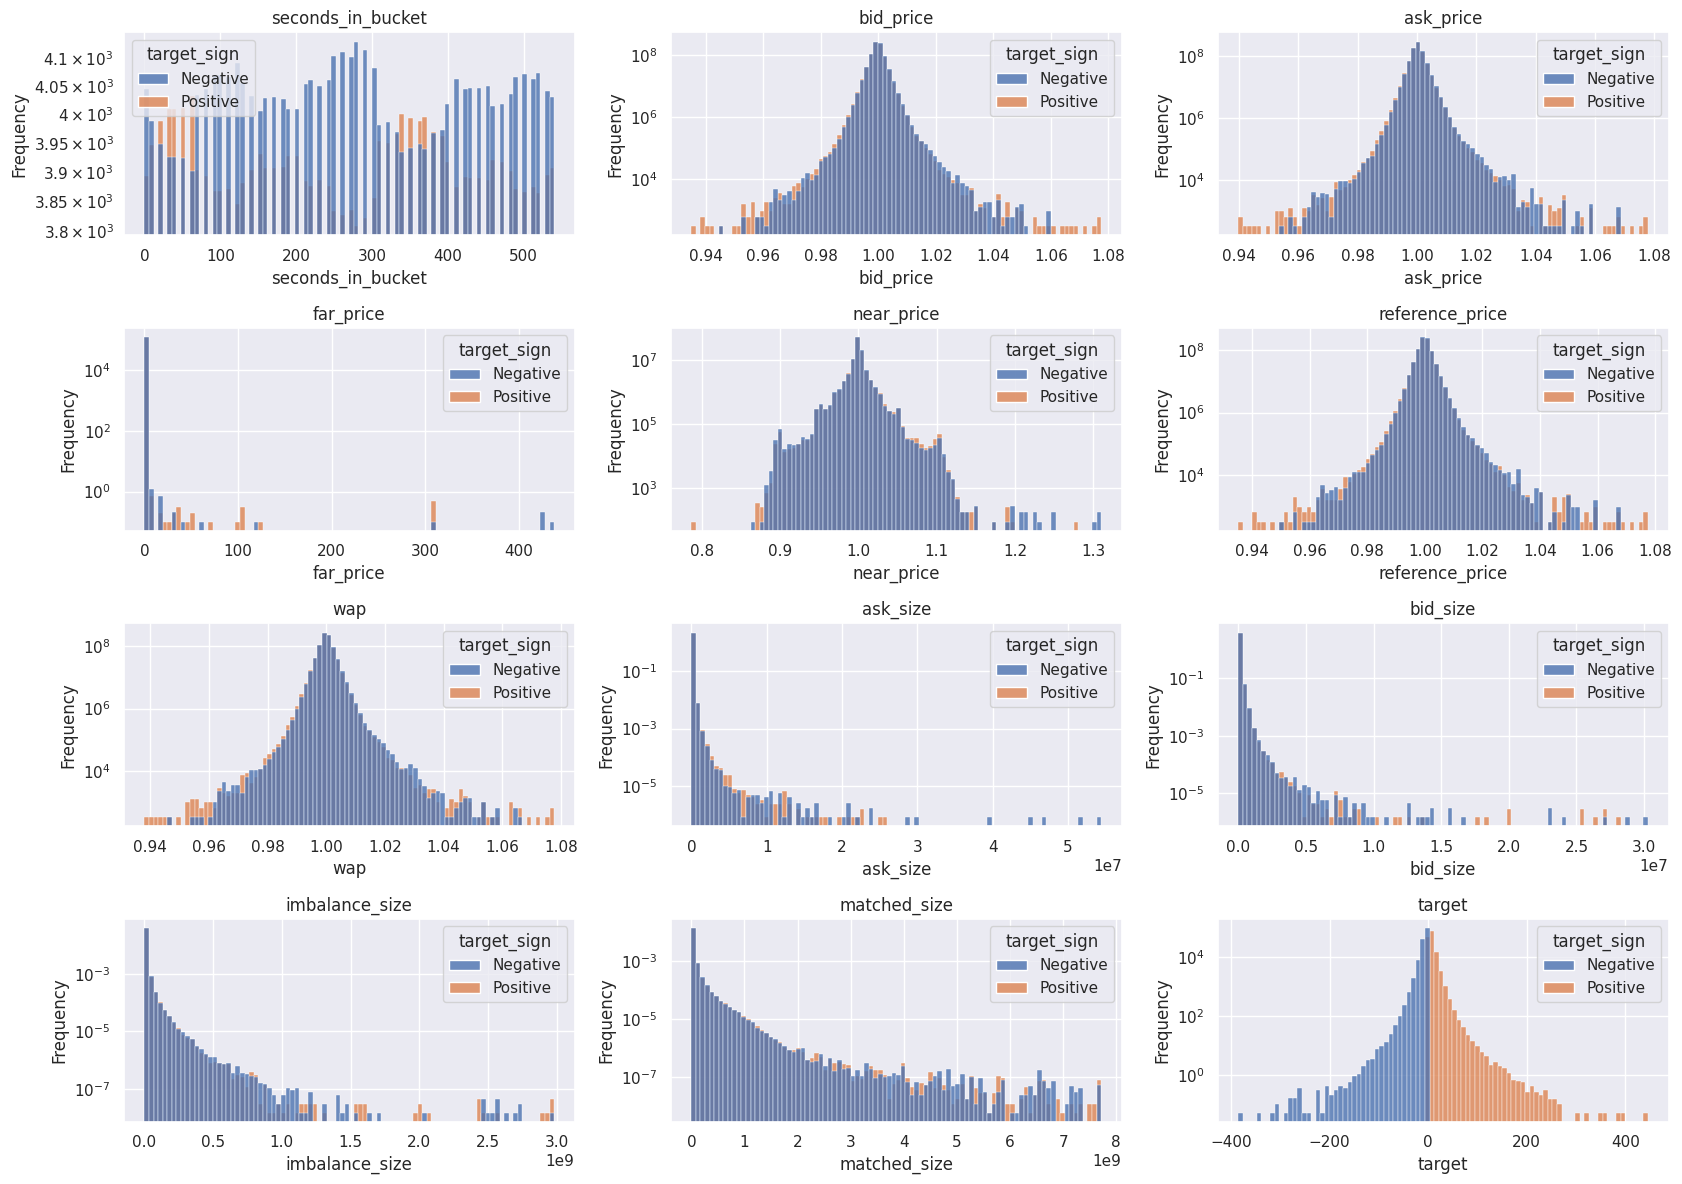
\includegraphics[width=1\linewidth]{images/Distribution.png}
  \caption{Comparative Distribution of Features under Positive and Negative Target Conditions}
  \label{fig:FeatureDistribution}
\end{figure}

The distribution of features across different target conditions demonstrates a notable similarity, characterized by nearly symmetrical patterns. Additionally, the data does not exhibit any issues of imbalance.

\noindent \textbf{Analyzing Single-Day Fluctuations in Features and Target for a Specific Stock}

\begin{figure}[H]
  \centering
  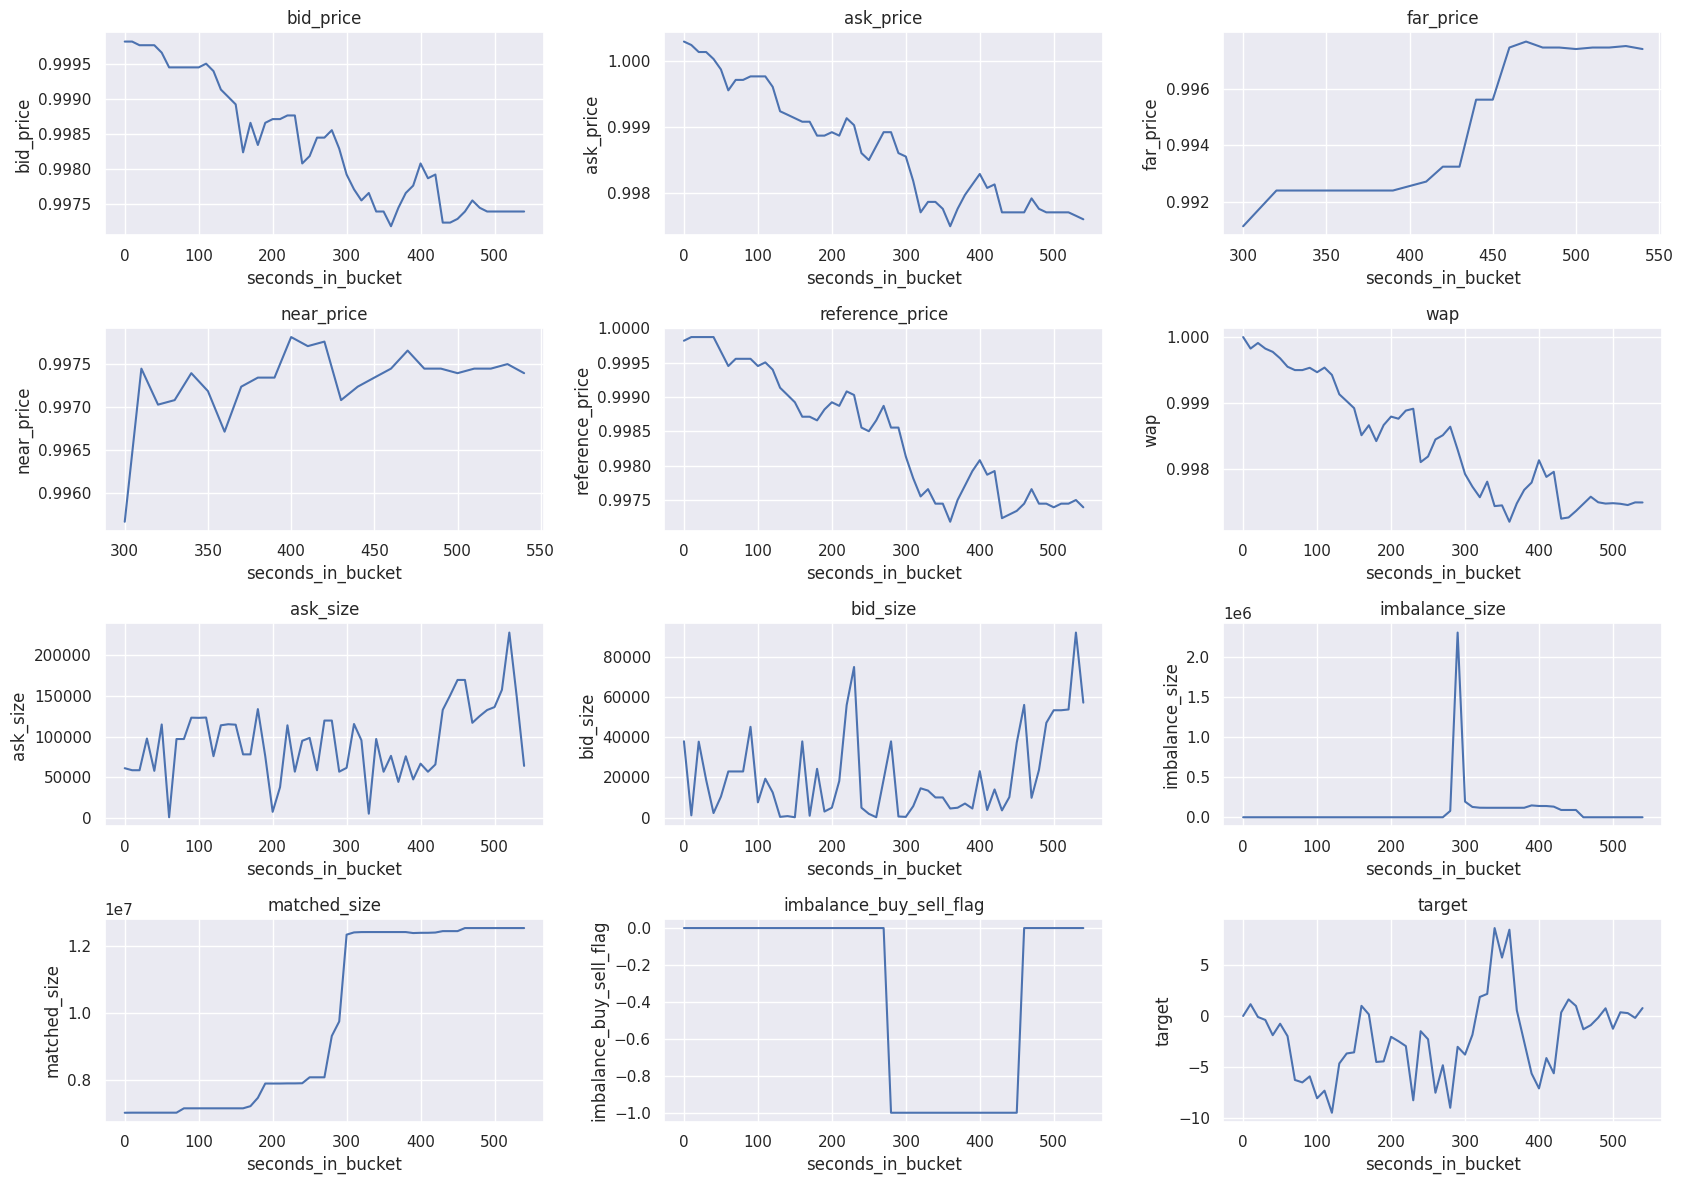
\includegraphics[width=1\linewidth]{images/LinePlot.png}
  \caption{Daily Movement Analysis of an Individual Stock}
  \label{fig:SingleDayMovement}
\end{figure}

In this analysis, it's evident that bid price, ask price, reference price, and weighted average price (WAP) exhibit a high degree of correlation. The far price and near price provide further insights into the dynamics of the closing auction order book and continuous trading order book, respectively. Notably, even in the absence of significant fluctuations in the continuous trading order book, there are observable spikes in both imbalance size and match size. These spikes indicate substantial shifts in the closing auction order book, which in turn trigger dramatic movements in the target, both upwards and downwards. Additional layers of information can be gleaned from examining the imbalance size, matched size, and the buy-sell imbalance flag.

\noindent \textbf{Scatter Plot Analysis of Features in Relation to the Target}

\begin{figure}[H]
  \centering
  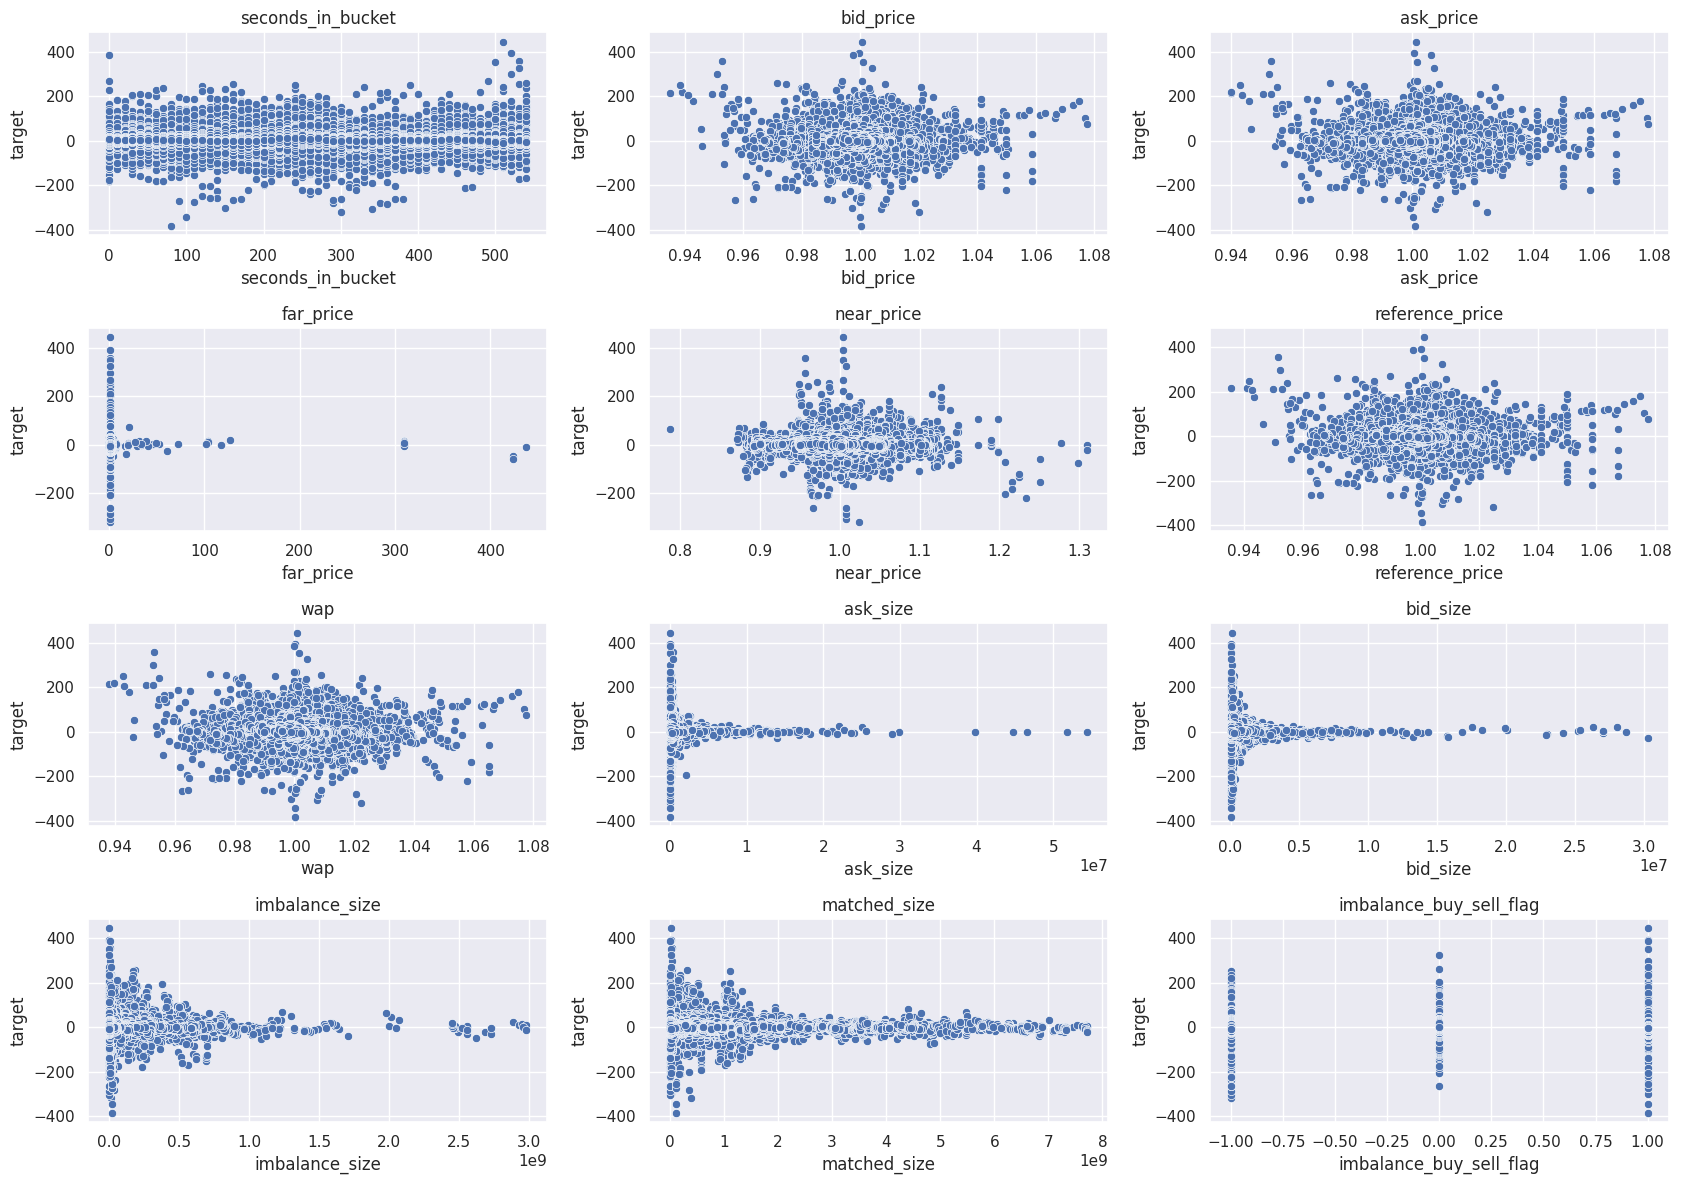
\includegraphics[width=1\linewidth]{images/Scatter.png}
  \caption{Correlation Scatter Plot Between Features and Target}
  \label{fig:FeatureTargetCorrelationScatter}
\end{figure}

The scatter plot sheds additional light on the relationship between features and the target. Despite the previously observed symmetrical distribution, this plot reveals distinct clusters. For variables like far price, ask size, bid size, imbalance size, and matched size, the majority of data points cluster around 0, where the target exhibits significant variability. Conversely, as these values increase, the variability of the target decreases, tending to fluctuate minimally around 0 within a narrow range.

\noindent \textbf{Analyzing the Correlation Between Features and Target}

\begin{figure}[H]
  \centering
  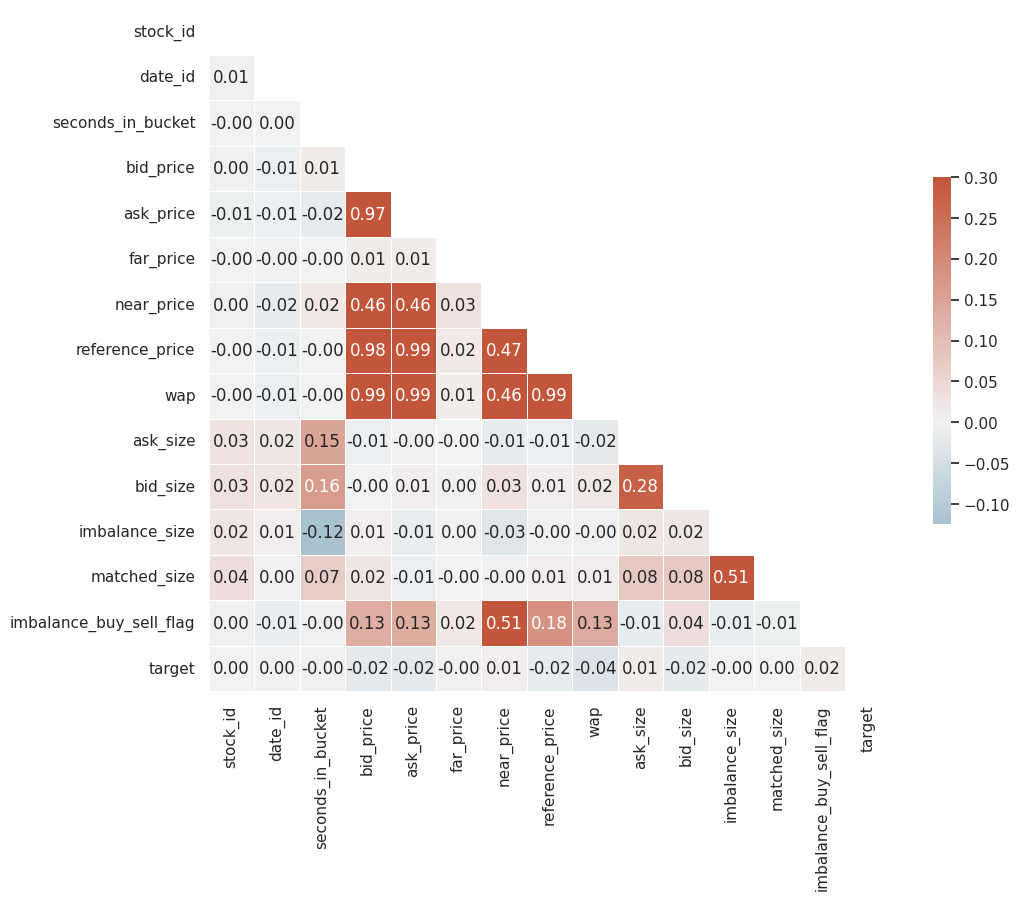
\includegraphics[width=1\linewidth]{images/CorrHeatMap.png}
  \caption{Heatmap Illustrating Correlation Between Features and Target}
  \label{fig:FeatureTargetCorrelationHeatmap}
\end{figure}

In this correlation analysis, various prices (ask price, near price, reference price, and WAP) demonstrate a high degree of correlation with one another, whereas far price exhibits a low correlation with these prices. This divergence is attributed to the fact that far price is derived solely from the closing auction order book information, which is not reflected in the continuous trading order book utilized by the other highly correlated prices.

Additionally, a strong correlation is observed between ask size and bid size, as well as between imbalance size and matched size. The imbalance buy-sell flag also shows a significant correlation with the near price, indicating that a positive flag often coincides with an upward trend in the near price. This phenomenon can be explained by the positive flag signaling a substantial number of unfilled bids, providing strong support against a price decline.

An intriguing aspect is the moderate correlation of sizes (ask size, bid size, imbalance size, and matched size) with seconds in the bucket. This correlation suggests varying market behaviors at different times of the day, such as increasing ask and bid sizes, decreasing imbalance size, and growing matched size as the day progresses.

However, a notable observation is that none of these features exhibit a high correlation with the target. This indicates the need for further feature engineering to extract more relevant information for better prediction accuracy regarding the target.

\subsubsection*{Advancements in Feature Engineering}

From the analysis, we can discern the distinct information each feature provides:
\begin{itemize}
  \item Ask price, near price, reference price, and WAP: Reflect continuous trading order book pricing.
  \item Ask size and bid size: Indicate continuous trading order book volumes.
  \item Far price: Represents closing auction pricing and volume data.
  \item Imbalance size, matched size: Blend of closing auction and continuous trading details.
  \item Second in bucket: Time-based information.
\end{itemize}

Here are some features I create from different perspective, aiming to extract useful infomation to predict target. About detialed implementation, please refer to my code.

\noindent \textcolor{brown}{\textbf{Single Stock Features}}

\begin{itemize}
  \item \textbf{Time-based Features:}
  \begin{itemize}
  \item \textit{date\_id\_week}: Captures the cyclic nature of the stock market on a weekly basis, using the modulo of the date ID to determine the day of the week.
  \item \textit{date\_id\_seconds}: Extracts the seconds component from the \textit{seconds\_in\_bucket} for more granular time analysis.
  \item \textit{date\_id\_minute}: Converts \textit{seconds\_in\_bucket} to minutes, offering a broader time perspective.
  \end{itemize}
  
  \item \textbf{Price Features:}
  \begin{itemize}
  \item \textit{spread}: Calculates the difference between ask and bid prices, indicative of market liquidity.
  \item \textit{spread\_ratio}: Evaluates the relative spread between ask and bid prices.
  \item \textit{mid\_price}: Represents the average of ask and bid prices, a typical measure of the market price.
  \end{itemize}
  
  \item \textbf{Volume Features:}
  \begin{itemize}
  \item \textit{total\_volume}: Sum of ask and bid sizes, reflecting the overall market volume.
  \item \textit{volume\_imbalance\_v1}: Ratio indicating the balance between bid and ask sizes.
  \item \textit{volume\_imbalance\_v2}: Ratio of ask size to bid size, another perspective on market balance.
  \item \textit{volume\_imbalance\_v3}: Direct difference between ask and bid sizes.
  \end{itemize}
  
  \item \textbf{Price Proximity Features:}
  \begin{itemize}
  \item \textit{near\_far\_ratio}: Ratio of near price to far price, indicating their relative positioning.
  \item \textit{near\_far\_imbalance}: Normalized difference between far and near prices.
  \item \textit{near\_far\_mid}: Average of near and far prices.
  \item \textit{near\_far\_spread}: Difference between far and near prices.
  \end{itemize}
  
  \item \textbf{Order Book Features:}
  \begin{itemize}
  \item \textit{auction\_volume}: Combined volume of imbalance and matched sizes from the auction.
  \item \textit{imbalance\_ratio\_v1}: Normalized difference ratio in the auction order book.
  \item \textit{imbalance\_ratio\_v2}: Ratio of imbalance size to total auction volume.
  \end{itemize}
  
  \item \textbf{Composite Features:}
  \begin{itemize}
  \item \textit{imbalance\_continuous\_ratio}: Links order book imbalance with total market volume.
  \item \textit{imbalance\_support\_v1, v2, v3}: Various measures combining spread with imbalance and volume metrics.
  \item \textit{depth\_pressure}: Interaction between volume imbalance and near-far price imbalance.
  \item \textit{market\_activity}: Measure of total market activity based on price and size.
  \item \textit{price\_volume\_imbalance\_v1, v2}: Ratios indicating the imbalance between bid and ask volumes weighted by price.
  \end{itemize}
  
  \item \textbf{Statistical Features:}
  \begin{itemize}
  \item Applying functions like mean, std, skew, and kurt to price and size arrays captures the statistical behavior of these features over time.
  \end{itemize}
  
  \item \textbf{Accumulative Features:}
  \begin{itemize}
  \item \textit{imbalance\_buy\_sell\_flag\_cumsum}: Cumulative sum of buy-sell flags, indicating the overall trend in buying or selling pressure.
  \item \textit{size\_according\_to\_flag\_cumsum}: Cumulative sum of sizes based on the buy-sell flag, providing a sense of directional volume accumulation.
  \end{itemize}
\end{itemize}


\noindent \textcolor{brown}{\textbf{Cross Sectional Features}}

\begin{itemize}
  \item \textbf{Cross-Sectional Statistics:}
  \begin{itemize}
  \item \textit{Cross Sectional Mean:} By calculating the mean of attributes grouped by date and time (seconds in bucket), these features represent the average market condition at a specific moment, providing a snapshot of typical market behavior.
  \item \textit{Cross Sectional Standard Deviation (std):} This metric measures the variability or spread of the attributes at each time point. A higher standard deviation indicates greater market volatility or divergence in trading behavior at that specific moment.
  
  \item \textit{Cross Sectional Skewness (skew):} Skewness assesses the asymmetry of the distribution of the attributes. This can indicate whether the market is leaning towards higher or lower values than the average at a particular time, which can be indicative of market sentiment or anomalies.
  
  \item \textit{Cross Sectional Rank:} Ranking the attributes in a percentile format within each group provides a relative standing of each stock or attribute at a particular time. This helps in identifying which stocks or attributes are performing better or worse compared to others in the same time frame.
  \end{itemize}

\end{itemize}


\noindent \textcolor{brown}{\textbf{Time Series Features}}
\begin{itemize}
  \item \textbf{Differential Features:}
  \begin{itemize}
  \item \textit{First and Second Order Differences (diff1, diff2):} These features capture the change in indicators over time, with \textit{diff1} representing the first-order difference (change from the previous value) and \textit{diff2} representing the second-order difference (change from the value before last). They help in identifying trends and reversals in time series data.
  \end{itemize}
  
  \item \textbf{Momentum Features:}
  \begin{itemize}
  \item \textit{Momentum (pct\_change):} The percentage change of indicators over time, this feature reflects the rate at which they are increasing or decreasing, akin to momentum in physics.
  \end{itemize}
  
  \item \textbf{Statistical Features:}
  \begin{itemize}
  \item \textit{Rolling Window Aggregations (mean, std, skew):} These features calculate the mean, standard deviation, and skewness of indicators over a rolling window. They provide a temporal view of the data, capturing trends, volatility, and asymmetry over specific time periods.
  \end{itemize}
  
  \item \textbf{Custom Statistical Features:}
  \begin{itemize}
  \item Functions like \textit{trend\_ratio, realized\_volatility, up\_var, down\_var,} and \newline \textit{calc\_autocorr} are applied to indicators over a rolling window to extract custom statistical insights, such as the direction of trends, volatility in upward and downward movements, and autocorrelation in the data.
  \end{itemize}
  
  \item \textbf{Correlation Features:}
  \begin{itemize}
  \item \textit{Correlation (compute\_corr\_numba):} This advanced feature calculates the pairwise correlation of selected indicators over a rolling window, providing insights into how different market variables move in relation to each other over time.
  \end{itemize}
  
\end{itemize}

\subsubsection*{Feature Selection}

Facing the challenge of Kaggle's RAM limitations and Optiver's extensive dataset with about 5 million data points, I encountered a significant hurdle: the construction of 204 features was consuming an enormous amount of RAM, rendering my model practically untrainable. It became imperative to devise strategies for selecting the most useful features for the next phase of training.

To tackle this, I turned to the method of Recursive Feature Elimination (RFE) with cross-validation, as proposed by \citep{guyon2002gene}, coupled with a basic XGBoost model. The core concept of RFE is to systematically build a model (in this case, XGBoost) and identify the most or least significant feature based on the feature importance scores generated by the model. This chosen feature is then removed, and the model is re-evaluated with the remaining features. This process is repeated until a pre-determined number of features is retained.

The procedure unfolds in the following steps:
\begin{itemize}
  \item Initial Model Training: Begin by training the XGBoost model with all available features in our dataset.
  \item Feature Ranking: Post-training, XGBoost ranks the features according to their importance in prediction accuracy.
  \item Elimination: Leveraging this ranking, RFE commences by discarding the least important feature(s) as indicated by the XGBoost model. Instead of selecting a fixed number of features to keep, cross-validation is employed to find the optimal count that maximizes model performance.
  \item Model Re-training: With a reduced feature set, the model undergoes re-training.
  \item Iteration: The cycle of eliminating features and re-training continues until we achieve the desired feature count.
\end{itemize}

After three rounds of this iterative process, I was able to reduce the feature count to 54, significantly shrinking the feature space dimension.

\section{Methods}


For my project, I plan to establish a foundational Elastic Net model initially. This approach employs a linear model augmented with regularization, specifically incorporating both L1 and L2 penalties. After setting this baseline, I aim to explore more advanced models, particularly focusing on tree-based boosting methods like LightGBM and XGBoost. I've chosen these models for their remarkable computational efficiency and proven effectiveness in managing large datasets, attributes crucial for the complexity and high-dimensionality typical of this project.

LightGBM and XGBoost are both variants of gradient boosting trees. Their methodology involves incrementally constructing the model by adding decision trees in a sequential manner. Each new tree specifically addresses and attempts to correct the errors made by its predecessors. This process utilizes gradient descent to optimize the loss function, continuously refining the model's accuracy. This technique is particularly valuable for tackling complex and challenging scenarios.

In addition to the aforementioned models, I am planning to incorporate a 'black box' model, specifically the Multilayer Perceptron (MLP), to more effectively capture the complex, non-linear patterns observed in the revised weighted average price (WAP) movements. The primary advantage of the MLP lies in its capability to unravel intricate patterns within data. This feature is particularly beneficial, as it offers a substantial edge over the more interpretable yet comparatively limited tree-based methods in certain contexts.

The MLP, a type of neural network, utilizes backpropagation for its training process. This involves employing algorithms like Adam or RMSprop for executing gradient descent. These algorithms are integral to the model's learning mechanism, as they iteratively minimize the loss function. They achieve this by adjusting the model's weights in accordance with the gradient of the loss function, ensuring a more effective and accurate learning process. For the implementation of the MLP, I will be using PyTorch\citep{paszke2019pytorch}, which is a highly acclaimed framework in the domain of deep learning, known for its flexibility and efficiency.

\subsection*{\href{https://en.wikipedia.org/wiki/Elastic_net_regularization}{Elastic Net}}

I chose Elastic Net\citep{zou2005regularization} as a starting point for my project due to its status as a quintessential linear model enhanced with regularization. This combination of L1 and L2 penalties makes it a robust baseline model, especially useful for dealing with issues of multicollinearity and overfitting, common in complex datasets. The training algorithm for Elastic Net involves a coordinate descent method, which iteratively optimizes the coefficients of the model. This process is relatively straightforward yet effective in handling both ridge (L2) and lasso (L1) penalties, striking a balance between feature elimination and weight shrinkage. The simplicity of its parameterization, coupled with the interpretability of a linear model, makes Elastic Net an attractive choice. Additionally, its implementation is well-supported by high-quality libraries like scikit-learn\citep{pedregosa2011scikit}, ensuring reliability and ease of use.

\subsection*{\href{https://lightgbm.readthedocs.io/en/stable/index.html}{LightGBM}}
LightGBM, developed by Microsoft\citep{ke2017lightgbm}, stands out due to its gradient-based one-side sampling and exclusive feature bundling. These techniques significantly enhance efficiency, particularly with large-scale data. The leaf-wise growth strategy, as opposed to the traditional level-wise approach, allows for more precise error correction. Its histogram-based optimization of the tree structure is not only memory efficient but also computationally faster, making it an excellent choice for handling sparse datasets, a frequent case in my project. LightGBM's approach to building trees and its efficiency in processing data make it a powerful tool in my modeling arsenal.

\subsection*{\href{https://xgboost.readthedocs.io/en/stable/}{XGBoost}}
XGBoost, conceptualized by Tianqi Chen\citep{chen2016xgboost}, operates on a similar gradient boosting framework but with distinct features. It employs regularized learning to prevent overfitting and effectively manages missing data, learning optimal imputation strategies. This characteristic is particularly vital given the nature of my dataset. XGBoost's standout feature is its capability for parallel computation across trees, significantly accelerating the training process. These features collectively ensure that XGBoost is not only robust in predictive performance but also efficient in handling complex data scenarios.

\subsection*{\href{https://en.wikipedia.org/wiki/Multilayer_perceptron}{Multilayer Perceptron}}
The MLP, a type of neural network, is recognized for its computational efficiency and straightforward yet effective parameterization. Despite its strength in capturing non-linear data patterns, the layered architecture of MLP can present challenges in interpretability. This is an important consideration for my project, and I intend to address it through using less layers to make it to be understood. The use of MLP in this project is particularly aimed at exploring deep, intricate relationships in the data that might not be readily apparent or captured by tree-based models.
\newline
\newline

In summary, my choice of algorithms, including Elastic Net, LightGBM, XGBoost, and MLP, is driven by their individual strengths and how they collectively offer a holistic understanding of the data. Elastic Net serves as a solid baseline with its regularization capabilities, effectively handling multicollinearity and overfitting. LightGBM and XGBoost excel in processing structured data, offering both efficiency and robustness, while MLP dives deep into modeling complex, non-linear relationships.

Leveraging Python libraries for these models enhances integration and experimentation, taking advantage of their extensive support and comprehensive documentation. With Elastic Net providing a clear interpretative foundation, I plan to balance the interpretability and complexity across all models. For the more intricate MLP, I'll take extra measures to ensure the outcomes are not only accurate but also interpretable, ensuring a nuanced understanding of the data.

\subsection*{Evaluation Metrics}

For the evaluation of the four models mentioned, I will use the \textbf{Mean Absolute Error (MAE)} as the key metric. MAE offers a straightforward and easily interpretable measure. It directly quantifies the average magnitude of errors in the same units as the dataset, which, in this context, relates to the basis points of stock price movements. This clarity in representation facilitates understanding across stakeholders with varying levels of technical knowledge.

MAE differs from the Mean Squared Error (MSE) in that it does not amplify the impact of outliers by squaring the errors. Financial datasets often contain outliers due to market fluctuations, news impacts, and other variables. MAE's resistance to outlier distortion makes it a more robust metric for these datasets.

Additionally, MAE is particularly suitable for non-linear models. Unlike MSE, MAE does not disproportionately escalate larger errors, which can be a byproduct of non-linear relationships in data.

However, for the MLP, I plan to use the \textbf{smooth L1 loss} instead of the standard L1 loss. This choice is motivated by the smooth L1 loss's ability to combine the advantages of L1 and L2 losses, offering a balance between sensitivity to outliers and smooth gradient descent. This hybrid approach is particularly beneficial for training neural networks like MLP, as it mitigates the potential issues of gradient explosion common with pure L1 loss while still retaining robustness against outliers.

To enhance interpretability, specific constraints have been applied to the models. For tree-based models, measures such as \textbf{limiting tree depth and introducing regularization to tree weights} are used. In contrast, for Neural Networks, I avoid imposing excessive restrictions that could undermine their capacity to model non-linearities. However, \textbf{control will be maintained over the network layers} to ensure a balance between model complexity and interpretability.


\section{Experiments}
\subsection{Hyperparameter Selection}

Given that my project involves a time series regression problem, it's crucial to handle the data splitting process with care. Random shuffling before splitting could lead to data leakage, which would adversely affect the model's performance. To avoid this, I adopt a time series split approach for cross-validation, as illustrated in the provided figure. This method ensures that the chronological order of the data is maintained, which is essential for time series analysis. I split the data into two parts, one is traing data which is used to train and validate our model, and the second serves for testing purposes.

\begin{figure}[H]
  \centering
  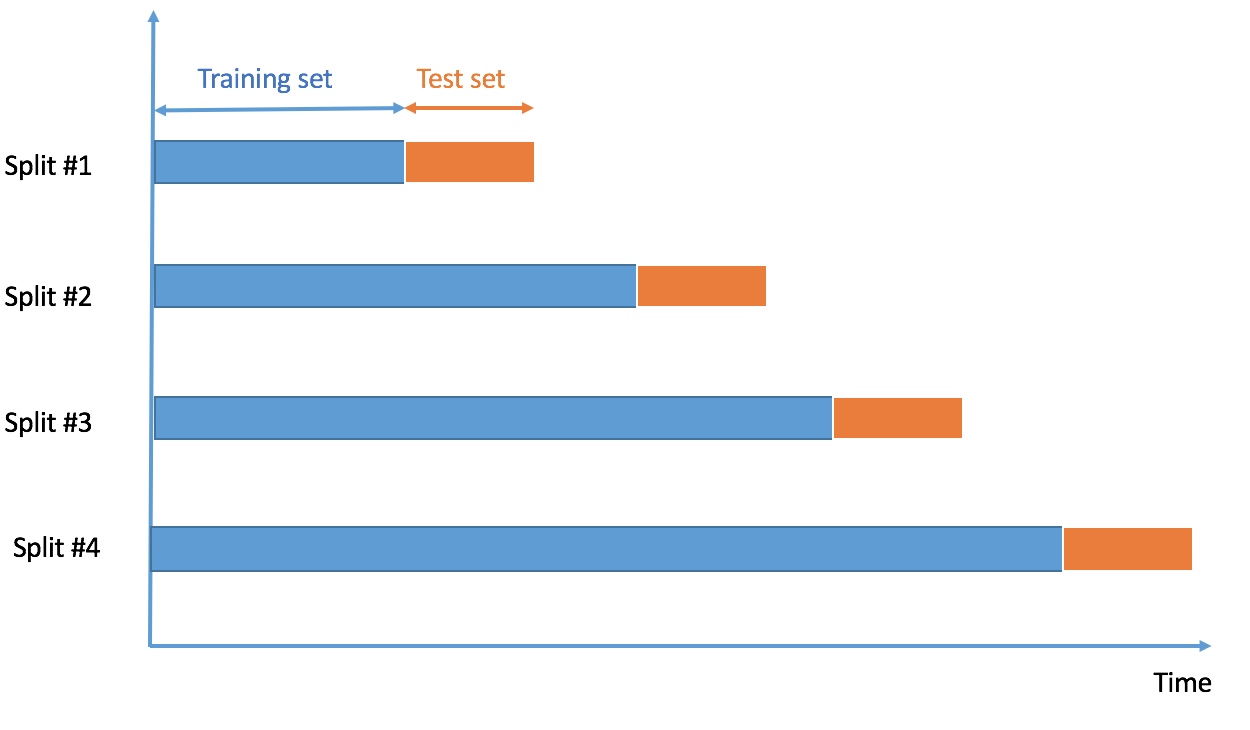
\includegraphics[width=0.7\linewidth]{images/TimeSeriesSplit.png}
  \caption{Time Series Split}
  \label{fig:TimeSeriesSplit}
\end{figure}

\subsubsection*{Elastic Net}
n tuning the Elastic Net model, I focus on three key parameters: alpha (L2 penalty), l1\_ratio (L1 penalty), and max\_iter (maximum number of iterations). The cross-validation process explores the following ranges for these parameters:
\begin{itemize}
  \item alpha: (0, 0.5, 1)
  \item l1\_ratio:(0, 0.5, 1)
  \item max\_iter: (100, 200, 500)
\end{itemize}
I simply use the \textbf{grid search} to find the best hyperparameters. Surprisingly, the optimal hyperparameters identified are alpha=0, l1\_ratio=0, and max\_iter = 100. At first glance, this result appears counterintuitive, as it suggests no regularization (penalty). However, I will later demonstrate that this configuration indeed delivers strong performance on the test set, underscoring the model's effectiveness even in the absence of conventional penalty parameters.

Here is the loss changing with max\_iter given different alpha and l1\_ratio:
\begin{figure}[H]
  \centering
  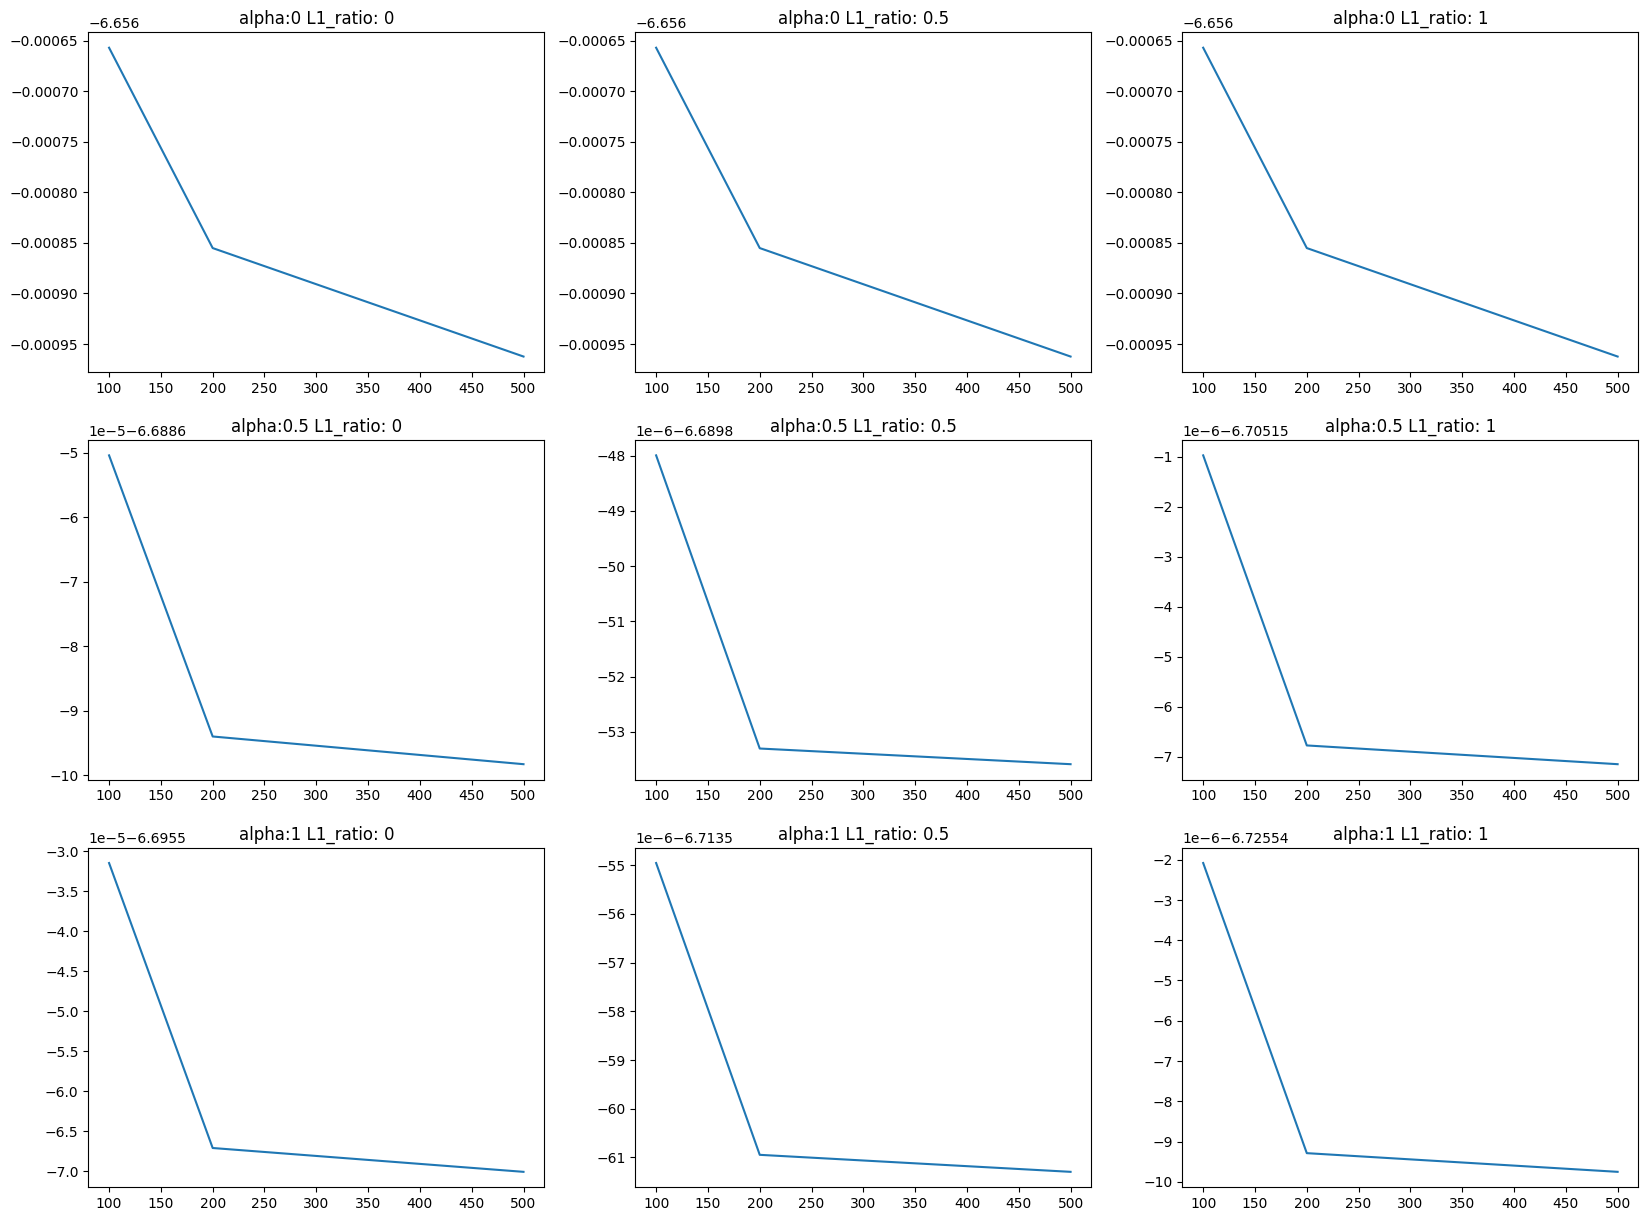
\includegraphics[width=1\linewidth]{images/cv1.png}
  \caption{cross-validation testing average loss}
  \label{fig:cv1}
\end{figure}

\subsubsection*{XGBoost}

Tuning hyperparameters for XGBoost, especially with a large dataset like this one, can be quite time-intensive. To streamline the process, I divided it into two distinct phases, acknowledging that certain hyperparameters have a more pronounced impact on the model's performance. In XGBoost, n\_estimators and learning rate are particularly influential.

In the first phase, I concentrated on these two key hyperparameters, as they are instrumental in determining how the model learns from data:
\begin{itemize}
  \item n\_estimators:  (50, 100, 200)
  \item learning\_rate: (0.01,0.1,0.3)
\end{itemize}

After this initial tuning, I determined that the optimal settings were 100 for n\_estimators and 0.1 for the learning rate. With these parameters fixed, I proceeded to the second phase of tuning.

The second phase involved fine-tuning parameters that help prevent overfitting, specifically max\_depth and colsample\_bynode:
\begin{itemize}
  \item max\_depth : (3, 6, 9),
  \item colsample\_bynode: (0.5, 0.65, 0.8)
\end{itemize}
The results from this phase indicated that the best configurations were a max\_depth of 6 and a colsample\_bynode of 0.8. This two-phase approach not only made the tuning process more manageable but also ensured a more focused and effective optimization of the XGBoost model.

\subsubsection*{LightGBM}

The process of tuning hyperparameters for LightGBM closely mirrors that of XGBoost, and I approached it in two distinct phases for efficiency and effectiveness.

In the first phase, my attention was primarily on the learning parameters:
\begin{itemize}
  \item n\_estimators:  (50, 100, 200)
  \item learning\_rate: (0.01,0.1,0.3)
\end{itemize}
From this phase, I found the optimal combination to be 100 for n\_estimators and 0.1 for the learning rate.

In the second phase, the focus shifted to parameters that help prevent overfitting:

At seond phase, I focus on parameters preventing model from overiftting:
\begin{itemize}
  \item num\_leaves: (30, 40, 50)
  \item colsample\_bytree:(0.5, 0.65, 0.8)
\end{itemize}
The best settings identified in this phase were 50 for num\_leaves and 0.5 for colsample\_bytree.

\subsubsection*{MLP}

When it comes to neural networks, hyperparameter tuning can be particularly time-consuming, a challenge compounded by the constraints of RAM and GPU availability, as well as the large size of the dataset. Given these limitations, I decided to focus on tuning just one key hyperparameter: the type of activation function.

I narrowed my choices down to two activation functions: ReLU and LeakyReLU. After conducting training and validation phases, I observed that the test loss with LeakyReLU was significantly lower compared to ReLU. Based on this finding, I have chosen to use LeakyReLU as the activation function in my neural network model. This decision is aimed at achieving better performance in terms of loss minimization, within the practical constraints of my computational resources.


\subsection{Results}

After training ElasticNet, XGBoost, LightGBM, and MLP with their respective tuned hyperparameters, the results clearly indicate varying levels of performance across these models. Here's a detailed look at the outcomes:

\begin{itemize}
  \item ElasticNet's testing MAE: 6.017632670611946
  \item XGboost's testing MAE: 5.970286832981401
  \item LightGBM's testing MAE: 5.971366890496566
  \item MLP's testing MAE: 6.959348124795339
\end{itemize}

\begin{figure}[H]
  \centering
  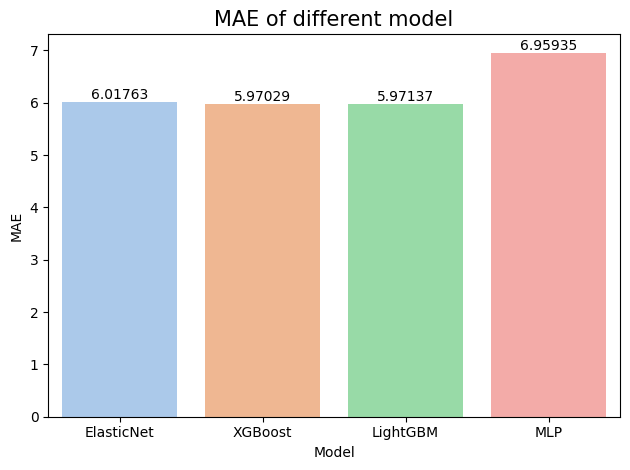
\includegraphics[width=0.7\linewidth]{images/res.png}
  \caption{MAE of different models}
  \label{fig:res}
\end{figure}

From these results, XGBoost emerges as the top performer in terms of test performance, closely followed by LightGBM, with a marginal difference in MAE. ElasticNet, while not matching the performance of the boosting models, still demonstrates respectable results. However, MLP lags behind, indicating that it may not be as effective for this particular dataset or problem.

The superior performance of XGBoost can be attributed to its efficient handling of structured data and its robustness in managing large datasets. Its gradient boosting framework, capable of sequentially correcting errors from previous trees, seems particularly effective in this scenario. On the other hand, the MLP's weaker performance could be due to its complexity and the potential for overfitting, especially when not all hyperparameters are exhaustively tuned due to resource constraints.

\subsection{Variable Importance Analysis}

\subsubsection*{Elastic Net}

The feature importance of linear model like Elastic Net could be represented as the weight of each feature. Here is th results:
\begin{figure}[H]
  \centering
  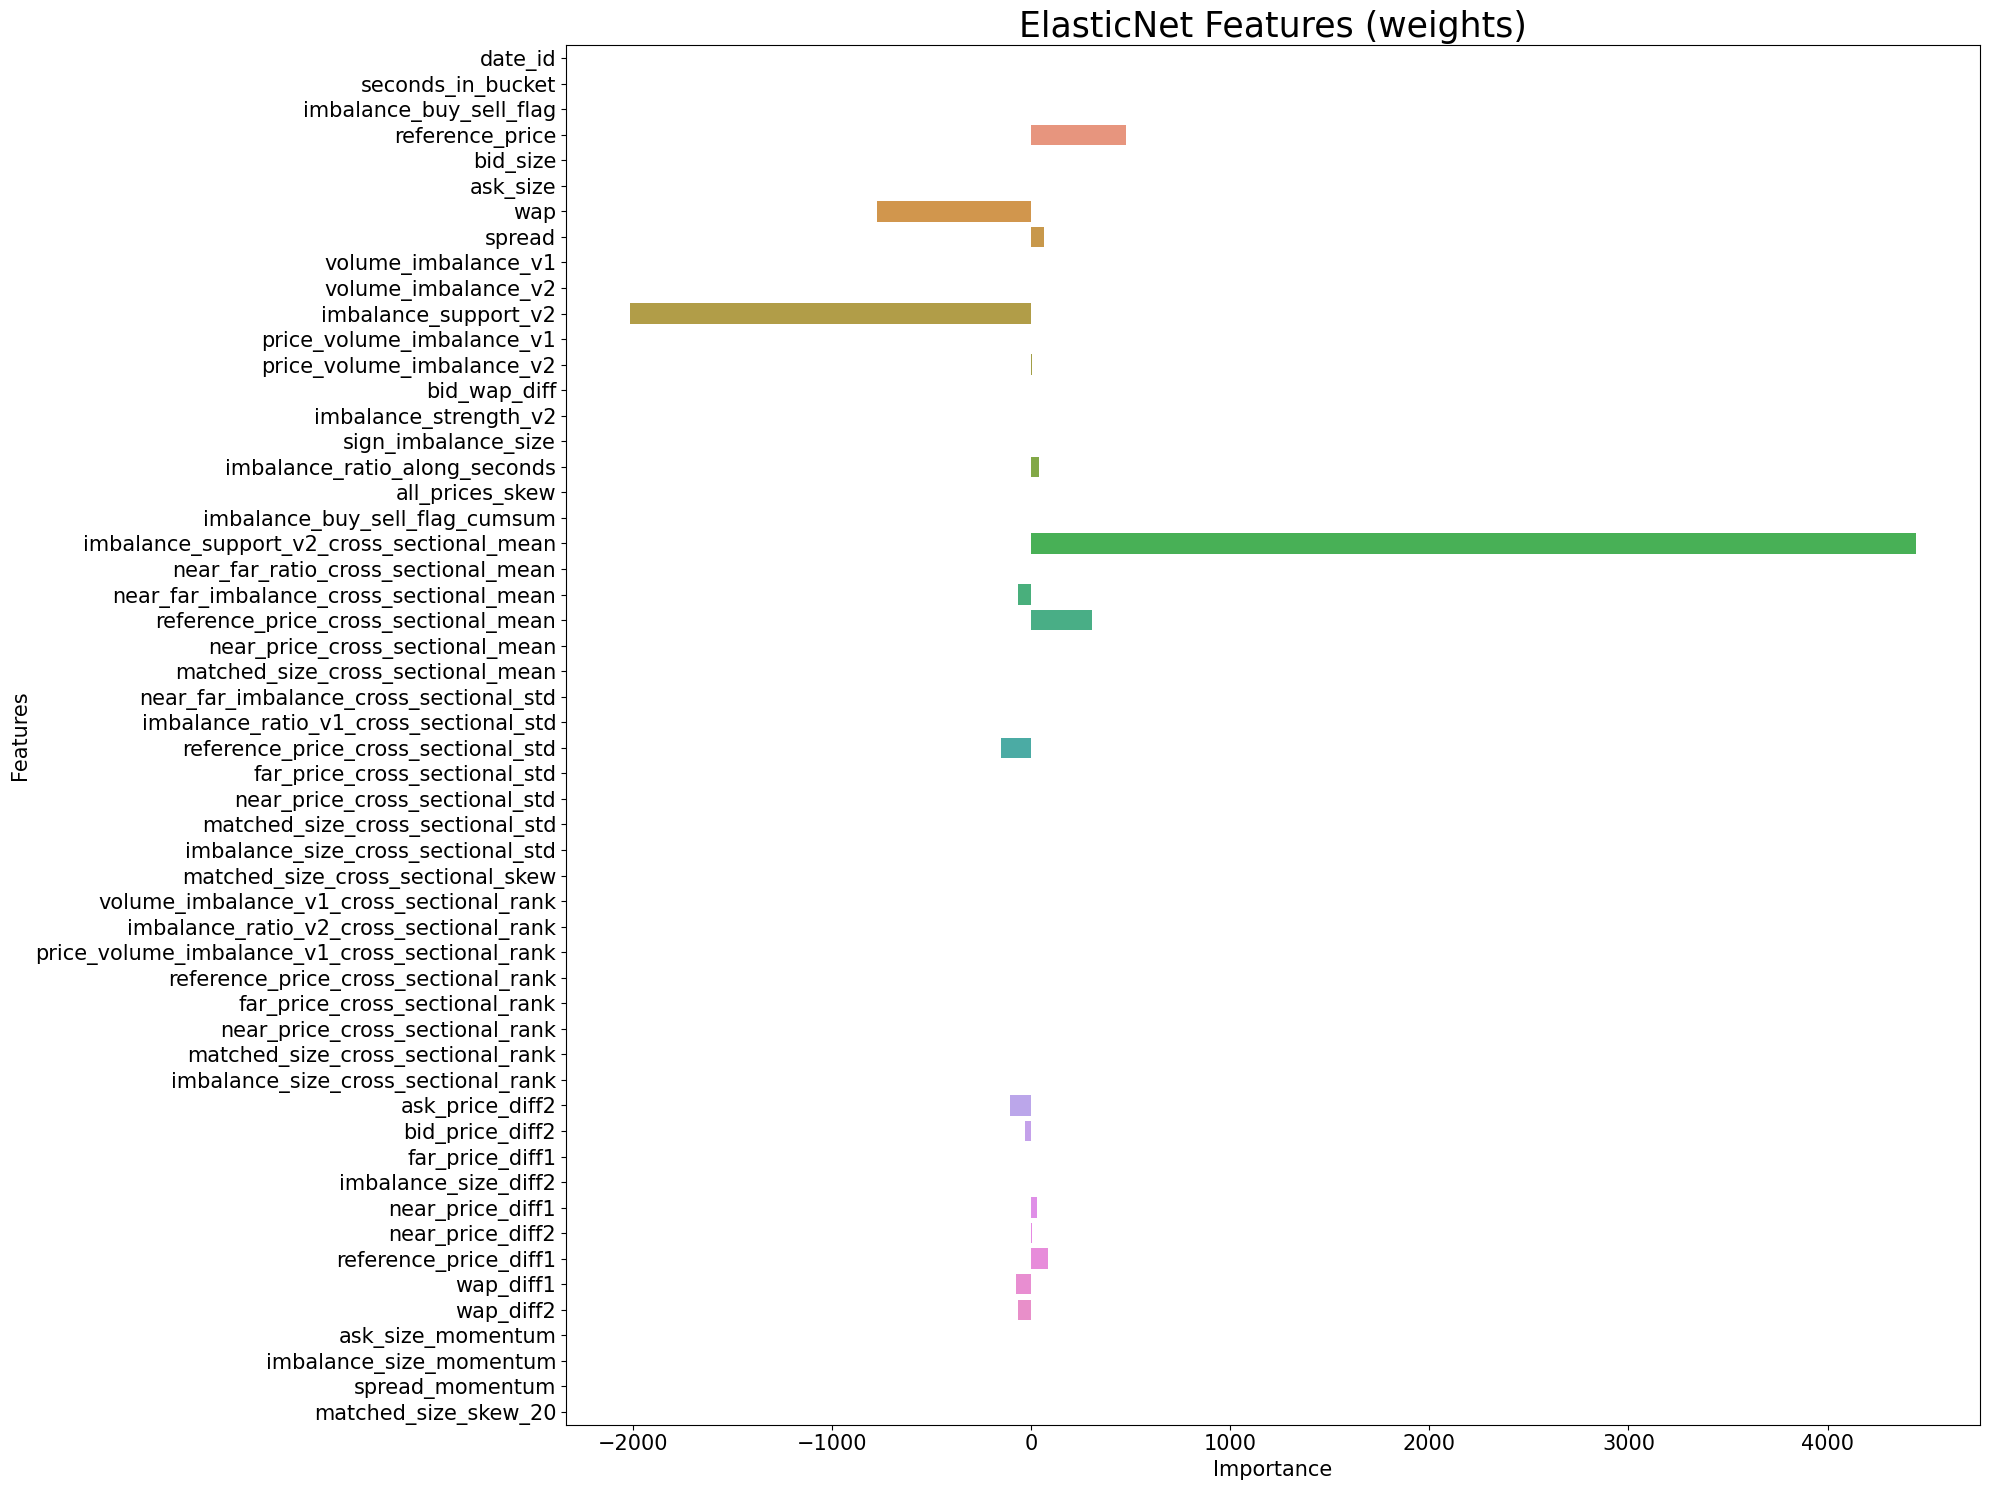
\includegraphics[width=1\linewidth]{images/ElasticNet_imp.png}
  \caption{Elastic Net Feature Importance}
  \label{fig:ElasticNet_imp}
\end{figure}
A longer bar indicates a higher importance, and the direction signifies whether the relationship is positive (to the right) or negative (to the left) with the target variable.
Here are some featues with high feature importance:
\begin{itemize}
  \item imbalance\_support\_v2\_cross\_sectional\_mean
  \item imbalance\_support\_v2
  \item wap
  \item reference\_price
  \item reference\_preice\_cross\_sectional\_mean
\end{itemize}

\subsubsection*{XGboost}

For XGBoost, there are several ways to indicate feature importance:
\begin{itemize}
  \item \textbf{Weight}: the number of times a feature appears in a tree. It tells us about the frequency of use.
  \item \textbf{Gain}: the average gain of splits which use the feature. It indicate indicates the quality of the splits using the feature.
  \item \textbf{Cover}: the average coverage of splits which use the feature where coverage is defined as the number of samples affected by the split. It shows the extent of impact a feature has on the data.
\end{itemize}

\noindent \textbf{Weight Importance}
\begin{figure}[H]
  \centering
  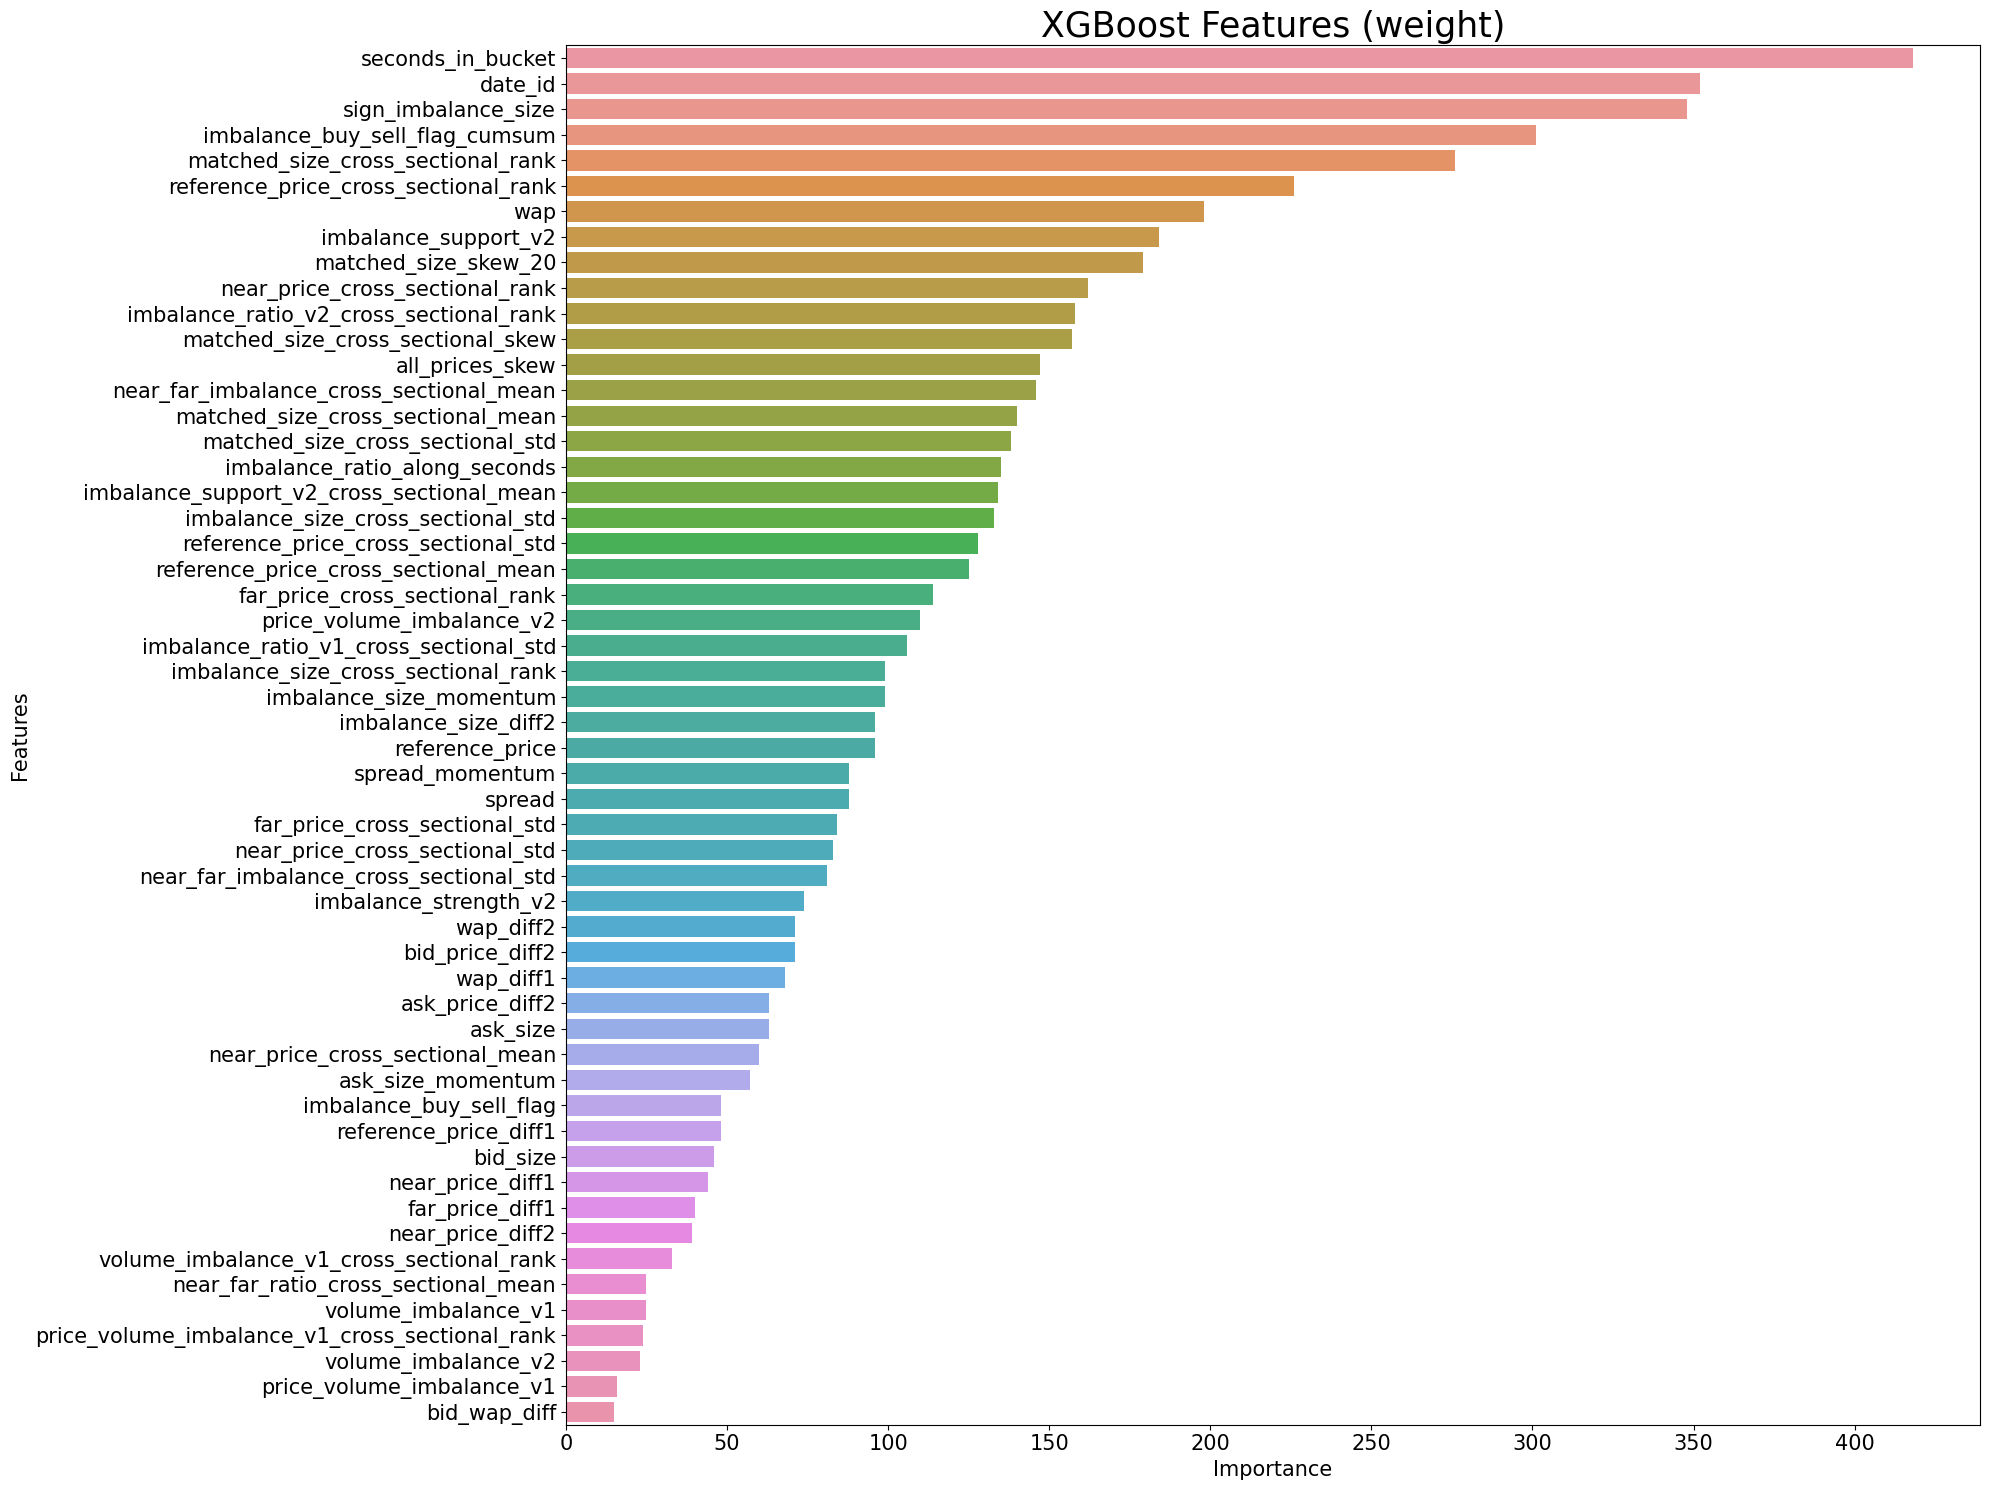
\includegraphics[width=1\linewidth]{images/xgb_weight.png}
  \caption{XGBoost Feature Importance (Weight)}
  \label{fig:xgb_weight}
\end{figure}

Considering the frequency aspect of feature importance, 'seconds\_in\_bucket' and 'date\_id' emerge as pivotal. This is because the market dynamics vary significantly over different times, and these features capture those temporal variations. 'Seconds\_in\_bucket' likely represents the time granularity of the data, indicating changes in market conditions within specific intervals, while 'date\_id' can be associated with broader date-specific trends or events. 

\noindent \textbf{Gain Importance}
\begin{figure}[H]
  \centering
  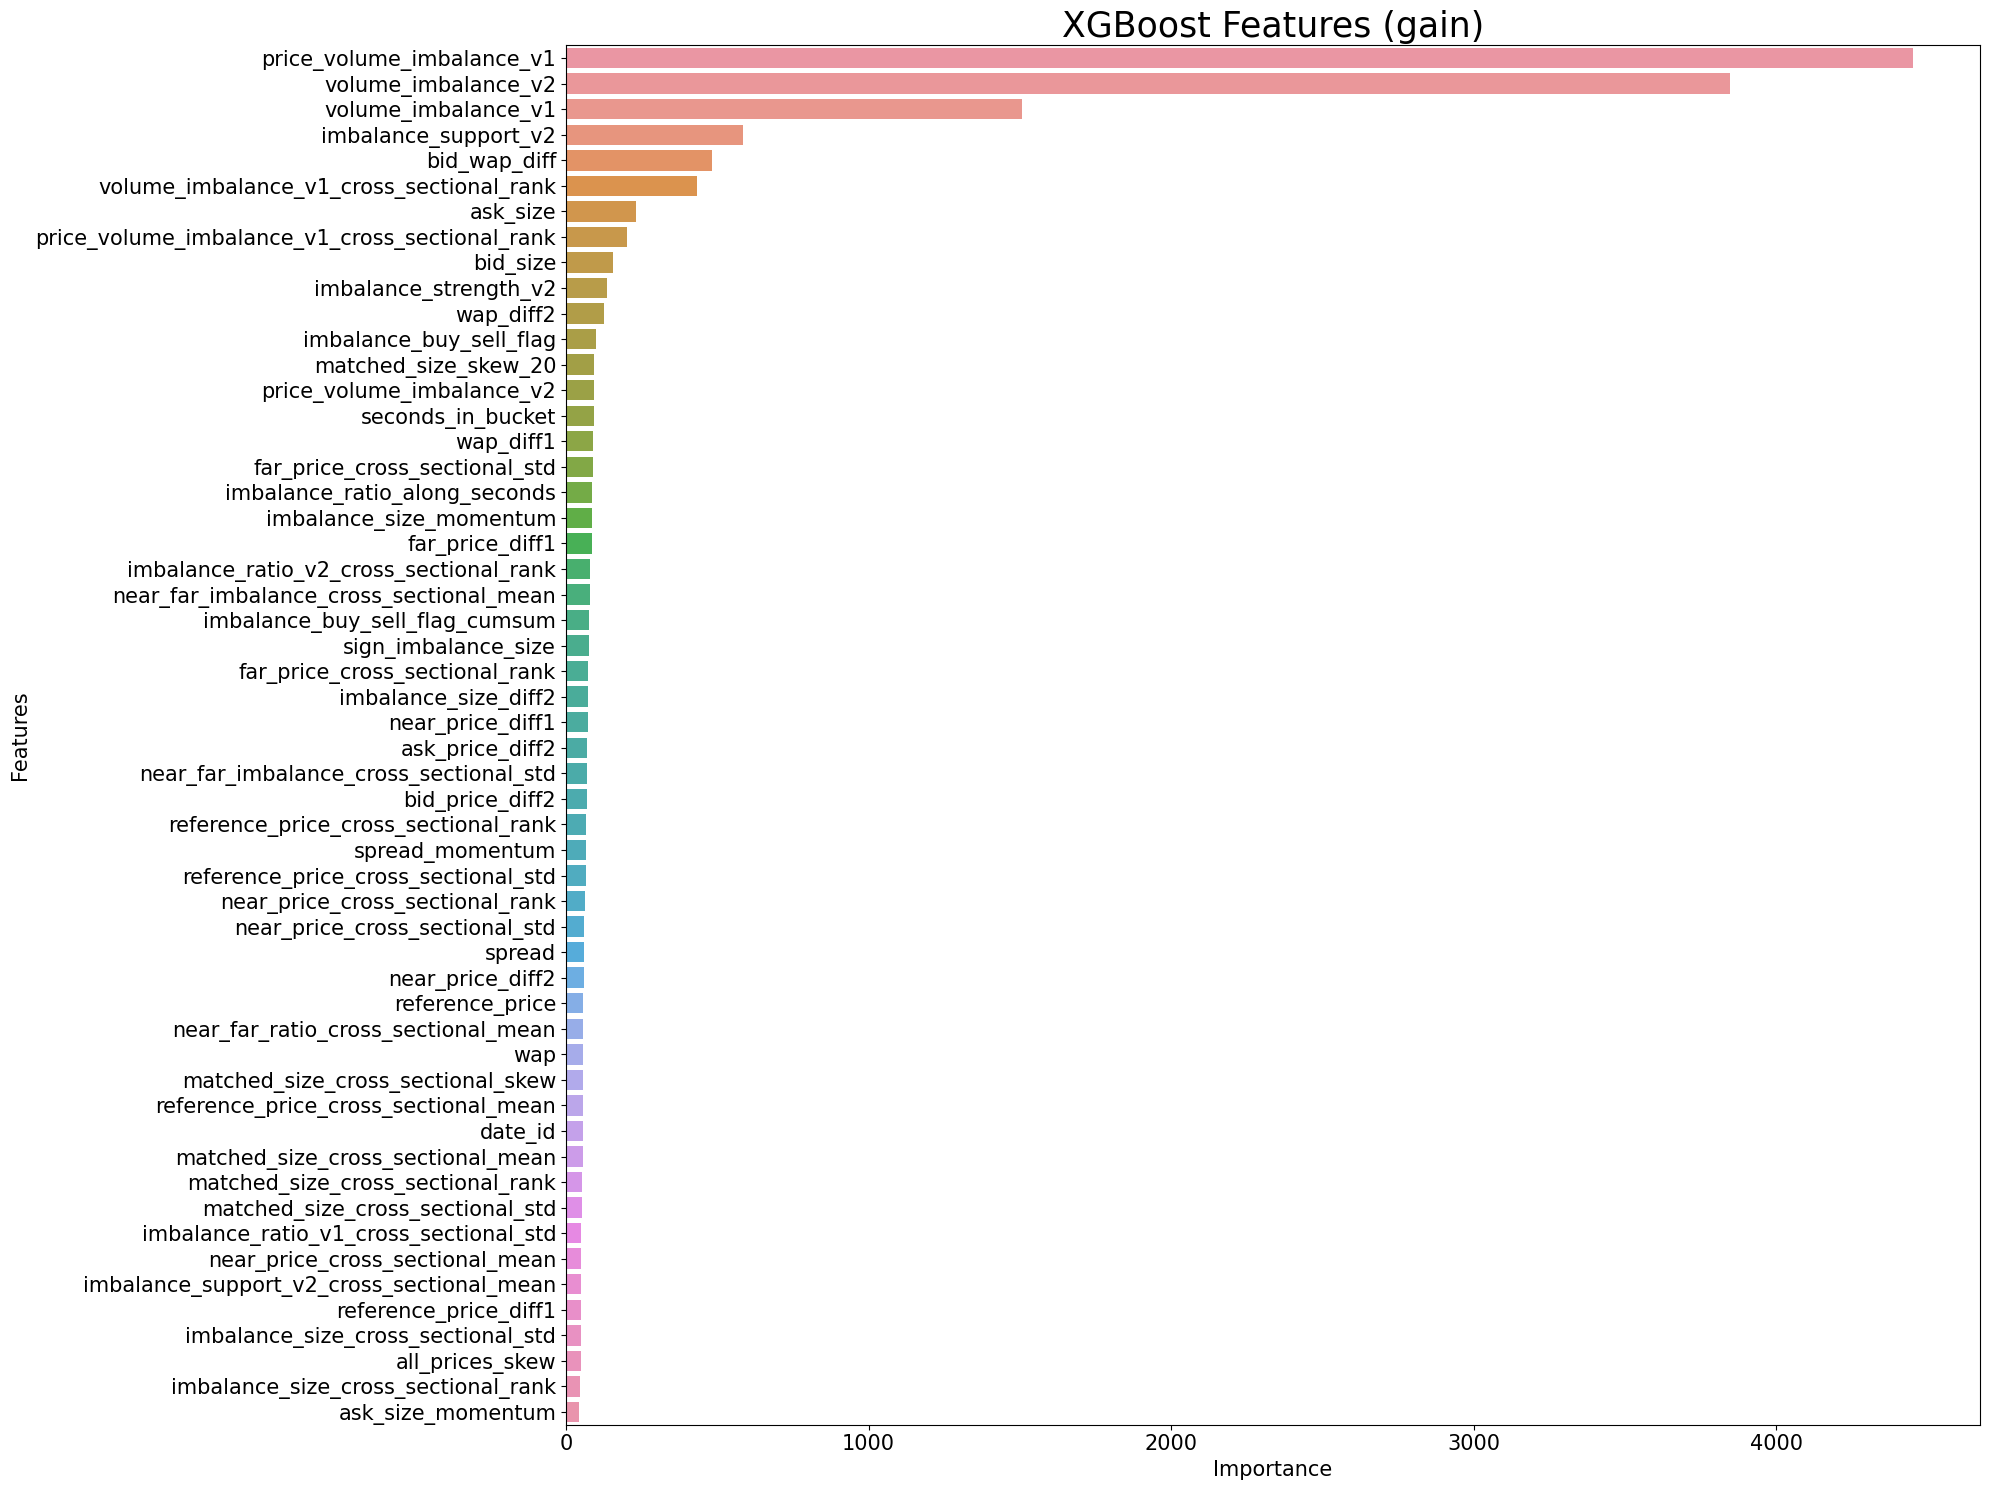
\includegraphics[width=1\linewidth]{images/xgb_gain.png}
  \caption{XGBoost Feature Importance (Gain)}
  \label{fig:xgb_gain}
\end{figure}
When evaluating feature importance from the perspective of splitting quality, a different picture emerges compared to the frequency-based view. In this context, the indicators of imbalance become highly significant. The most substantial gains are observed from features related to price and volume imbalances, suggesting that these factors are crucial in improving the model's predictive accuracy. Such indicators likely capture critical market conditions that influence price movements, making them valuable for the model's decision-making processes.
\newline

\noindent \textbf{Cover Importance}
\begin{figure}[H]
  \centering
  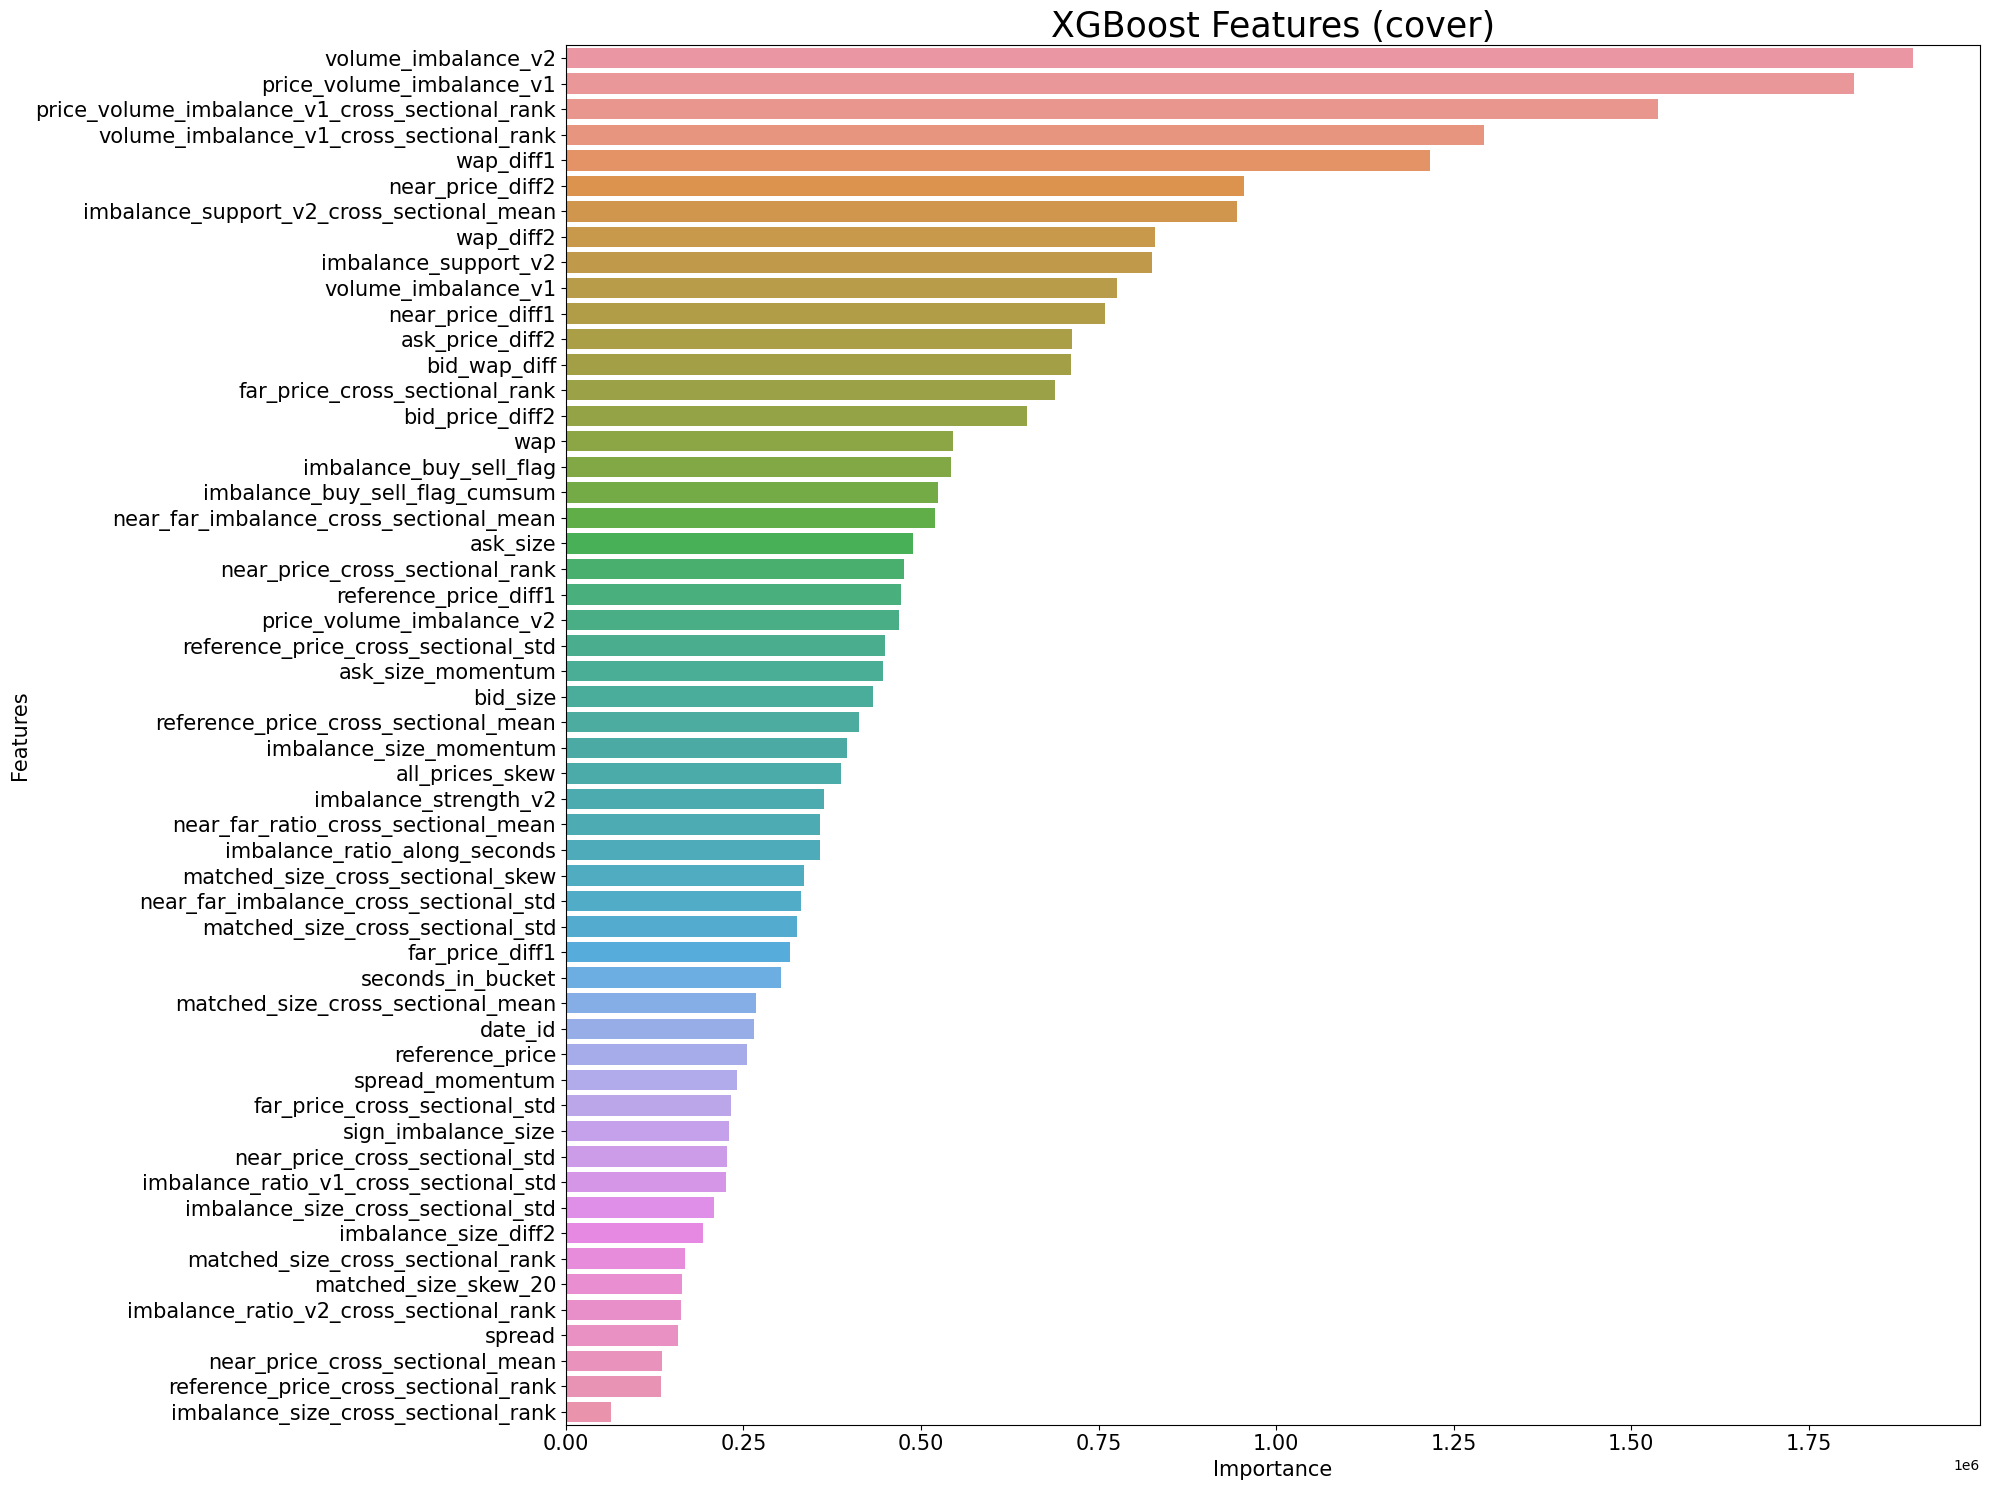
\includegraphics[width=1\linewidth]{images/xgb_cover.png}
  \caption{XGBoost Feature Importance (Cover)}
  \label{fig:xgb_cover}
\end{figure}

Regarding cover-based feature importance, the observations closely align with those derived from gain importance. Once again, the imbalance indicators stand out as pivotal elements. This similarity indicates that features which provide the greatest gain—improving the model's predictions when used in splits—also tend to affect a large number of observations, thereby reinforcing their significance in the model's decision-making process.

\subsubsection*{LightGBM}

LightGBM also provides different versions of feature importance:

\begin{itemize}
  \item \textbf{Split}: This metric counts the number of times a feature is used to split the data across all trees.
  \item \textbf{Gain}: This represents the cumulative gains from all splits that the feature contributes to. 
\end{itemize}

These metrics are closely aligned with those used by XGBoost.

\noindent \textbf{Split Importance}
\begin{figure}[H]
  \centering
  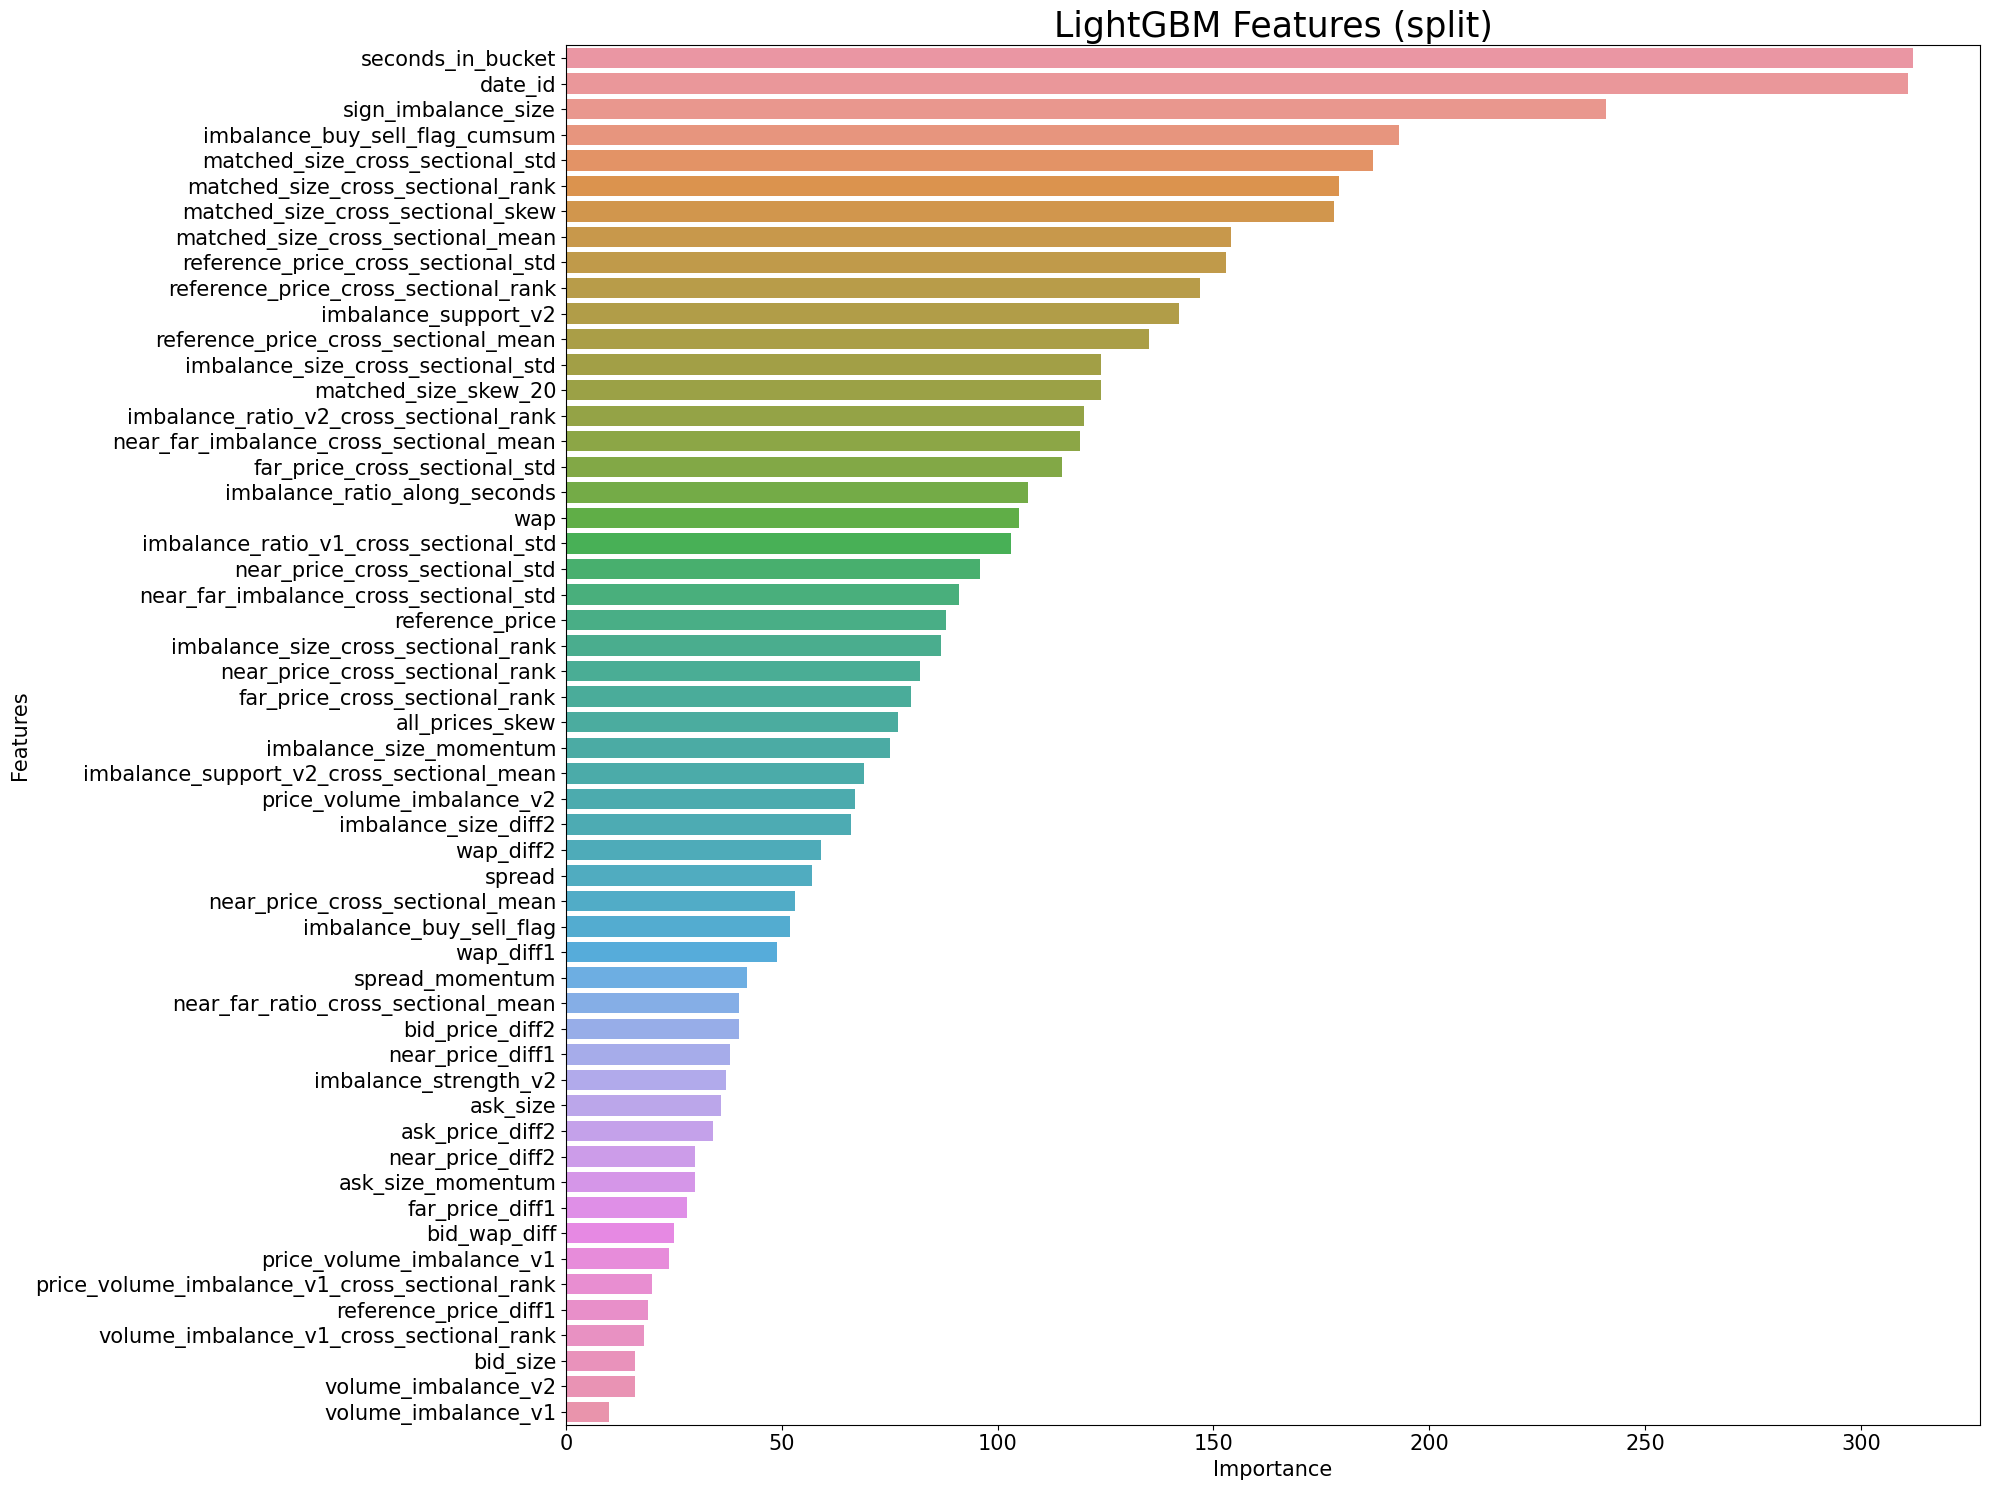
\includegraphics[width=1\linewidth]{images/lgb_split.png}
  \caption{LightGBM Feature Importance (Split)}
  \label{fig:lgb_split}
\end{figure}
The Split Importance results from LightGBM exhibit similarities to the Weight metric of XGBoost, yet there are subtle differences. For instance, the cross-sectional standard deviation of matched size stands out as a significant feature in LightGBM, which is not as prominent in XGBoost.

\noindent \textbf{Gain Importance}
\begin{figure}[H]
  \centering
  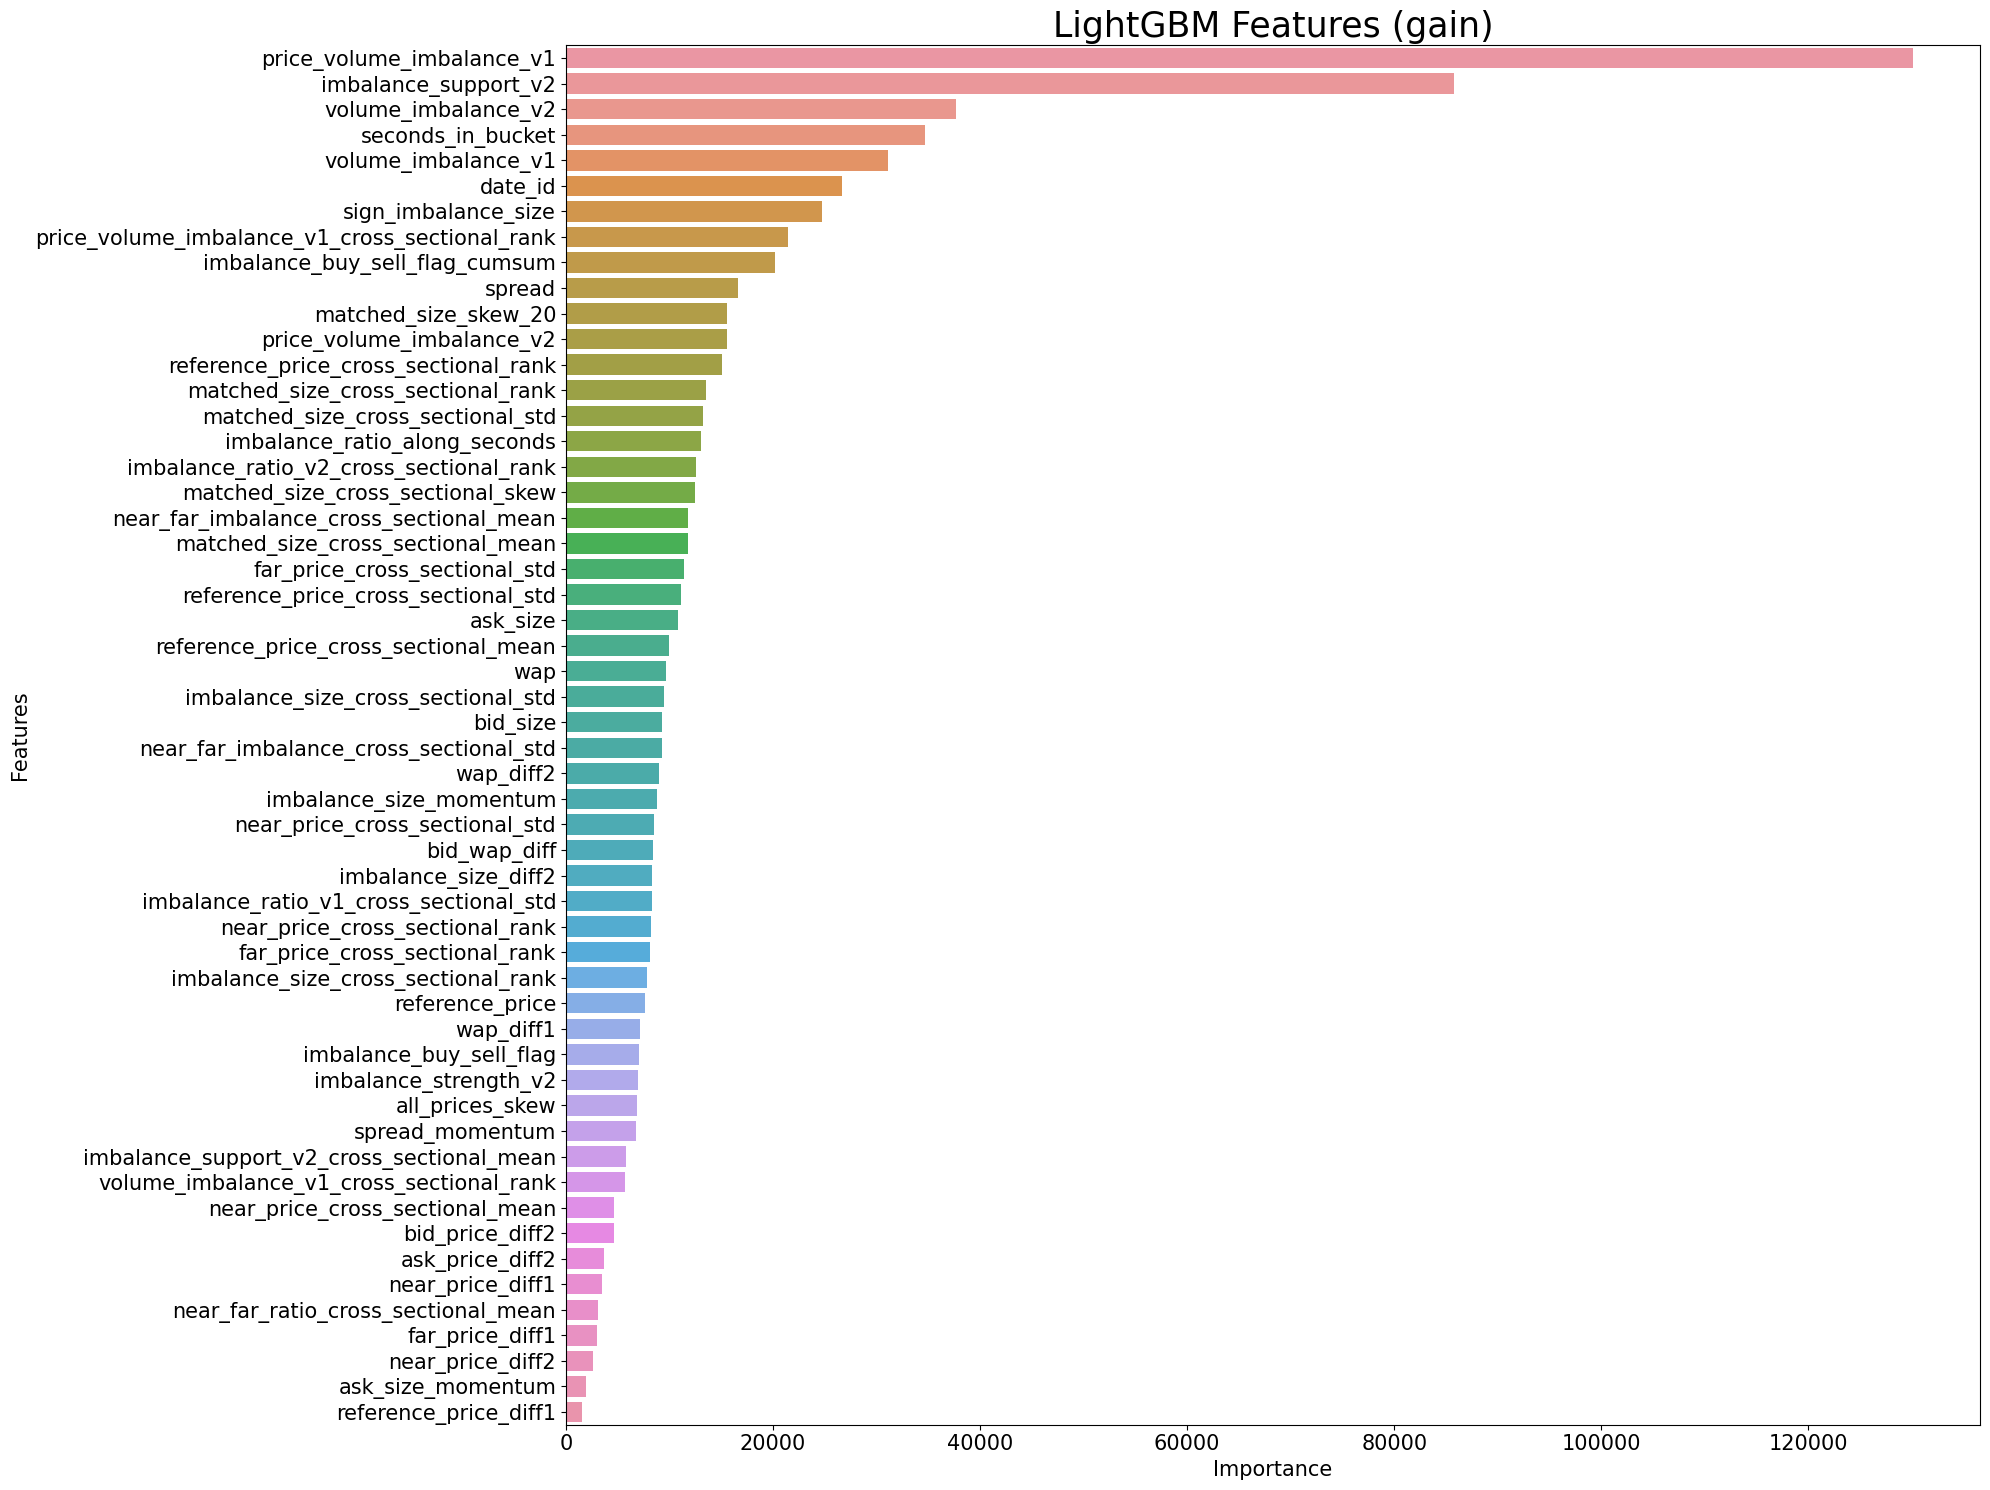
\includegraphics[width=1\linewidth]{images/lgb_gain.png}
  \caption{LightGBM Feature Importance (Gain)}
  \label{fig:lgb_gain}
\end{figure}

When examining the gain metric in LightGBM, it is evident that both the imbalance indicators and time-related features are of great importance. This suggests that the model significantly benefits from features that capture market imbalances as well as those that reflect the temporal aspects of the data, enhancing its predictive accuracy.


\subsubsection*{Conclusion}

The significance of various features can vary across different models. Nevertheless, within the boosting framework, particularly in models like LightGBM and XGBoost, the feature importances align closely, with only nuanced differences. In this project, the boosting methods predominantly leverage imbalance and time features to grasp the nuances of market dynamics. On the other hand, the linear model, such as Elastic Net, seems to place a higher emphasis on price information to make predictions.


\section{Insight}
\begin{enumerate}
  \item \textbf{Unexpected Importance of Time Variables}: The significant role of 'seconds\_in\_bucket' and 'date\_id' in the XGBoost and LightGBM models initially caught me off guard. Intrigued by this, I delved into research and literature\citep{selccuk2006intraday}, which clarified that intraday time dynamics play a critical role in stock movements, especially in the closing minutes of trading. This knowledge helped me understand the crucial impact of time-sensitive factors like closing auctions and last-minute trades on stock prices.

  \item \textbf{Dominance of Imbalance Indicators}: Discovering the prominent role of imbalance-related features such as imbalance\_size and imbalance\_buy\_sell\_flag in the models was a revelation. Since high-frequency trading was a new territory for me, I turned to academic literature on market microstructure\citep{o1998market}\citep{o2015high} to comprehend this phenomenon. It was fascinating to learn how liquidity, often quantified through imbalance metrics, is a pivotal factor in high-frequency trading and prediction.
  
  \item \textbf{Dataset Gaps and Potential Enhancements}: The moderate performance of the MLP model compared to the tree-based models indicated possible limitations in the dataset's ability to capture complex, non-linear relationships. This finding suggests the need for more diverse features or alternative data sources to better represent the nuanced aspects of market dynamics, a direction I plan to explore in future iterations of the project.
  
  \item \textbf{Trade-offs Between Interpretability and Accuracy}: The project underscored the delicate balance between model complexity and interpretability. Complex models like MLPs, though potentially more adept at identifying intricate patterns, suffer from a lack of transparency. This experience has reinforced my appreciation for more interpretable models like Elastic Net, especially in scenarios where clear understanding of variable influences is crucial for informed decision-making and meeting regulatory requirements.
\end{enumerate}


\section{Errors and Mistakes}

\begin{enumerate}
  \item \textbf{Navigating Kaggle's 30GB RAM Limitation}: One of the first hurdles I encountered was the 30GB RAM limitation on Kaggle. Working within this constraint while handling extensive datasets was like trying to fit a square peg in a round hole. It demanded a lot of ingenuity and optimization of code to ensure everything ran smoothly without hitting the memory ceiling.

  \item \textbf{Dealing with a Large Dataset}: The sheer size of the dataset presented its own set of challenges. It felt like maneuvering a tanker ship – every move required careful planning and consideration. Handling such a massive dataset efficiently required not just computational resources, but also a strategic approach to data processing and management.
  
  \item \textbf{Time-Consuming Hyperparameter Tuning}: Tuning hyperparameters, especially given the size of the dataset and Kaggle's RAM restrictions, was a test of patience. It was akin to finding a needle in a haystack, where each tweak could lead to significantly different outcomes. This part of the project was both meticulous and time-intensive.
  
  \item \textbf{Feature Engineering and Selection}: The process of feature engineering and selection was another time-intensive task. It was like assembling a jigsaw puzzle, where each piece (feature) had to be carefully examined and placed to form a coherent picture (model). Balancing the inclusion of informative features against the risk of overfitting or introducing noise was a continuous exercise in discernment.
  
  \item \textbf{MLP Structure Design}: Designing the MLP structure was perhaps the most challenging part of the project. It was a process of trial and error, experimenting with various structures only to find that the complexity didn't necessarily translate to better performance. After several days of tweaking and testing different configurations, I decided to revert to a simpler MLP structure. This decision, though initially seeming like a step back, was a valuable learning experience in understanding the nuances of neural network architecture.
\end{enumerate}

However, despite the challenges, I found ways to streamline the process and make it more efficient. One key strategy was employing Numba for feature calculation, which significantly sped up the computation. It was like finding a turbo button in a complex video game - suddenly, everything moved faster and more smoothly. This approach not only saved time but also allowed me to focus on other critical aspects of the project.

% \section*{Citations}
\bibliography{citation}


\end{document}
